%%--------------------Chapter 3------------------------
\chapter{How I Built It} \label{chap:thetis_design}

\section{Stakeholders} \label{sec:stakeholders}
As with any project, stakeholders are a crucial part of the design process.
Stakeholders drive overarching requirements that the device must achieve in order to be accepted for operation.
On an individual level, the committee overseeing this thesis are the major stakeholders as they have a vested interest in the success or failure of the project.
However, some organizational-level stakeholders have also expressed interest in the project and provided some additional requirements.
A summary of the stakeholders is provided in Table \ref{tab:stakeholders}.

\begin{table}
	\caption{A summary of stakeholders of the Thetis device}
	\label{tab:stakeholders}
	\centering
	\begin{tabular}{|p{0.3\linewidth} | p{0.6\linewidth}|}
		\hline
		\rowcolor[gray]{0.8}
		\multicolumn{1}{|c|}{\textbf{Stakeholder}} & \multicolumn{1}{|c|}{\textbf{Description}} \\
		\hline
		Committee members & Individual professors who have expressed interest in the project and have agreed to assist in its development. Specifically, Dr. Wood and Dr. Weaver would like to deploy Thetis on university projects; Dr. Gutierrez has provided many requirements on the performance of the instrumentation; and Dr. Silaghi is interested in its application to autonomous navigation. \\
		\hline
		Florida Institute of \newline Technology & The university has several classes and projects where Thetis could be useful. The Instrumentation Design and Analysis class used Thetis as a demonstrator for designing PCBs and field experiments. Thetis was also designed with Surf Engineering Analysis in mind for students to have a new open source sensor to experiment with. \\
		\hline
		NSWC Carderock - \newline Combatant Craft Division (CCD) & This three-letter agency of the government has expressed interest in using Thetis as a testing and evaluation tool for small unmanned crafts \\
		\hline
	\end{tabular}
\end{table}

\subsection{Hands-On Users} \label{ssec:hands_on_users}
Thetis is intended to be used by college students that are at least sophomore-level and have a basic understanding of instrumentation and electronics.
The device is simple to use, requiring the user to flick a switch to turn it on or off, and then press a physical or digital button to start or end logging.
Thetis is also designed to accommodate advanced users who need to leverage different features of the device for their research or want to tinker with it.
It can also be used by laboratory technicians and instrumentation engineers to aid with data-collection experiments for tracking three dimensional bodies

\section{Design Rationale} \label{sec:design_rationale}
Thetis is envisioned as an open-source all-in-one inertial data logging solution for use in research projects.
The device incorporates multiple sensors, GPS tracking, and a WiFi-capable microcontroller in order to enable as many features as can be envisioned by the end users.
One of the driving considerations was the small footprint.
Thetis Revision F is designed to fit into one of the smallest IP67-rated enclosures available on the market [LINK].  
This tiny form factor allows it to be inconspicuously mounted to any floating body like surfboards, scale models, or wave buoys without upsetting their inertial characteristics or impeding nominal operation.

\subsection{Problem Description} \label{ssec:problem_desc}
I originally envisioned Thetis as the solution to a couple of problems I encountered during my undergraduate studies.
For my fluid mechanics laboratory section, we conducted an experiment where we needed to track the rolling of a model pontoon boat as we adjusted its center of gravity.
Because the lab lacked any way to directly measure the body's inertial movement, angle gauges were placed on the hull and the students had to conduct a time motion analysis from a video recording to plot the roll angle frame-by-frame.
This was inefficient and made me start thinking about how this could be improved.

The second problem occurred in a class the following semester where we deployed surf boards and pressure gauges into the ocean to monitor a surfer's ride along a wave.
We used two different instruments, the Lowell MAT-1 data logger [CITE - LOWELL], and an iPhone 6 inside a life proof case.
The Lowell instrument was not designed for this use case.
First, the sensor board is housed within a cylindrical body, making properly alignment to a Cartesian (square) coordinate system almost impossible.
Second, the sensor only had an accelerometer and magnetometer on board.
It reported roll, pitch, and yaw but the roll and pitch were derived from tilt and gravitational acceleration and the magnetometer determined yaw.
These values assumed the sensor would be in the vertical position, and we used it in a horizontal position.
Suffice to say, we were not using the Lowell properly and could not get reliable or useful information out of it for our analysis.

The iPhones were much better suited as they had a full 9-DOF IMU sensor suite and a great data logger application to get the raw sensor values and sensor fusion results.
However, since this was a class comprised of inexperienced undergraduates, we didn't often check that the seal on the phone cases were properly set before going into the water.
Within a matter of months, both iPhones were lost because students removed the case and did not replace the water-tight gasket, costing a large sum of money.

Given my experience with these classes, it was clear to me that a low-cost inertial data logging solution could be valuable to the department as a teaching and laboratory instrument.

\subsection{Mission Statement} \label{ssec:mission_statement}
Thetis aims to democratize the inertial measurement and tracking space for small scale experiments by implementing an open-source, feature-rich, all-in-one solution to monitoring the movements of bodies.

\subsection{Stakeholder Requirements} \label{ssec:stakeholder_reqs}
Interviews with the stakeholders occurred over several months and informed a set of requirements that they determined were necessary for the project's success.
These overarching requirements were placed into a traceability matrix (Table \ref{tab:stakeholder_reqs_traceability}) to track their priority and status throughout the project.

\begin{table}
	\centering
	% \fontsize{10pt}{10pt}\selectfont
	\renewcommand{\arraystretch}{1.75}
	\caption[Stakeholder Traceability Matrix]{A slimmed down traceability matrix for the stakeholder requirements. Verification and Validation status is not shown here. The priority of each requirement is the relative weight of requirement compared with all others.}
	\begin{tabular}{|c | p{0.5\textwidth} | c | c | c |}
		\hline
		\textbf{ID} & \multicolumn{1}{c |}{\textbf{Description}} & \textbf{Weight} & \textbf{Priority} & \textbf{Status} \\
		\hline
		SR 01 & The system shall be able to record acceleration, rotation rate, orientation, and position & 1 & 14 & TIP \\
		SR 02 & The system shall be able to fit into a small IP67-rated, or better, enclosure & 1 & 14 & D \\
		SR 03 & The system shall be able to be powered by battery for more than 4 hours continuously & 1 & 14 & A \\
		SR 04 & The system shall be cheaper than \$200 per unit & 0.4 & 6 & A \\
		SR 05 & The system shall use components that are readily available COTS & 1 & 14 & D \\
		SR 06 & The system designs shall be open source for modification by students & 0.7 & 10 & D \\
		SR 07 & The system shall allow users to change settings via interface and/or configuration file & 0.7 & 10 & D \\
		SR 08 & The system shall communicate extra-device using WiFi and USB & 0.3 & 4 & A \\
		SR 09 & They system shall have enough on-board storage for 4 hours of continuously logging at 64 Hz & 1 & 14 & TIP \\
		\hline
	\end{tabular}
	\label{tab:stakeholder_reqs_traceability}
\end{table}

\subsection{Risk Identification} \label{ssec:risk_identification}
The following tables explore some of the larger risks associated with each of the stakeholder requirements.
Risks are categorized into several types: Technical, Cost, Schedule, Organizational, and Operational.
Each risk has an associated consequence on the project's development and a severity rating from "Low" to "High".
With every risk, we can apply a mitigation to it to reduce the severity of the consequence.

\paragraph*{Technical Risks} These are risks that pose a technical challenge to the project such as sensor accuracies, programming difficulty, or component specifications. 
These risks are likely to impede the development of Thetis by showing up during testing and forcing workarounds after the fact, rather than before.

\paragraph*{Cost Risks} These risks pose a threat to Thetis's development budget.
They are more likely to manifest in the supply chain of Thetis, especially in the wake of the COVID-19 pandemic and the chaos of the chip shortage.

\paragraph*{Schedule Risks} By delaying the program's development, Schedule Risks are the most notorious and costly.
These risks manifest as delays in development or the supply chain and can significantly impact the expected delivery time of the device.
They also are prominent across all phases of the design process from planning to testing and are only mitigated, but never eliminated during the design process.

\paragraph*{Organization Risks} The stakeholders represent various organizations that have an interest in Thetis.
This risk type poses a problem for the specific stakeholder organization and their interests.
This can be viewed from the political, economical, or temporal points of view as these are important considerations for the stakeholders.

\paragraph*{Operational Risks} These risks challenge end users of the device while they are testing.
Most of them can be mitigated in the design process by working directly with the end users and ensuring their concerns are met.
However, the majority of them will only manifest during testing and must be mitigated after the fact.
This could mean substantial cost increases and schedule delays depending on the severity of the risk.

\begin{landscape}


% ==================================
% === STAKEHOLDER REQUIREMENT XX ===
% ==================================


% \paragraph*{SR XX} - 

% {\fontsize{8pt}{8pt}\selectfont
% \begin{longtable}{| p{0.12\linewidth} | p{0.16\linewidth} |  p{0.20\linewidth} | p{0.08\linewidth} | p{0.20\linewidth} | p{0.08\linewidth} |}
% 	\hline \endlastfoot
	
% 	\hline
% 	\rowcolor[gray]{0.8}
% 	\multicolumn{6}{|c|}{ } \\
% 	\hline
% 	\textbf{Stakeholder:} & \multicolumn{5}{|l|}{} \\
% 	\hline
% 	\textbf{Rationale:} & \multicolumn{5}{|p{0.8\linewidth}|}{} \\
% 	\hline
% 	\textbf{Fit Criterion:} & \multicolumn{5}{|p{0.8\linewidth}|}{} \\
% 	\hline
% 	\rowcolor[gray]{0.8}
% 	\multicolumn{6}{|c|}{ } \\
% 	\hline
% 	\textbf{Risk} & \textbf{Risk Issue} & \textbf{Risk Consequence} & \textbf{Initial Risk} & \textbf{Risk Mitigation} & \textbf{Risk \newline After \newline Mitigation} \\
% 	\hline
% 	Technical \newline Assessment &  &  & \cellcolor{} &  & \cellcolor{} \\
% 	\hline
% 	Cost \newline Assessment &  &  & \cellcolor{} &  & \cellcolor{} \\
% 	\hline
% 	Schedule \newline Assessment &  &  & \cellcolor{} &  & \cellcolor{} \\
% 	\hline
% 	Organizational \newline Assessment &  &  & \cellcolor{}  &  & \cellcolor{}  \\
% 	\hline
% 	Operational \newline Assessment &  &  & \cellcolor{} &  & \cellcolor{}
% 	\label{tab:sr01_feasibility}
% \end{longtable}
% }
% \newpage


% ==================================
% === STAKEHOLDER REQUIREMENT 01 ===
% ==================================


\paragraph*{SR 01} - The system shall be able to record acceleration, rotation rate, orientation, and position

{\fontsize{8pt}{8pt}\selectfont
\begin{longtable}{| p{0.12\linewidth} | p{0.16\linewidth} |  p{0.20\linewidth} | p{0.08\linewidth} | p{0.20\linewidth} | p{0.08\linewidth} |}
	\hline \endlastfoot
	
	\hline
	\rowcolor[gray]{0.8}
	\multicolumn{6}{|c|}{ } \\
	\hline
	\textbf{Stakeholder:} & \multicolumn{5}{|l|}{Thesis Committee} \\
	\hline
	\textbf{Rationale:} & \multicolumn{5}{|p{0.8\linewidth}|}{The system needs to be able to record the inertial characteristics of a floating body} \\
	\hline
	\textbf{Fit Criterion:} & \multicolumn{5}{|p{0.8\linewidth}|}{This will be accomplished using a 9-DOF IMU and GPS receiver with accuracies not to exceed one standard deviation of a reference source} \\
	\hline
	\rowcolor[gray]{0.8}
	\multicolumn{6}{|c|}{ } \\
	\hline
	\textbf{Risk} & \textbf{Risk Issue} & \textbf{Risk Consequence} & \textbf{Initial Risk} & \textbf{Risk Mitigation} & \textbf{Risk \newline After \newline Mitigation} \\
	\hline
	Technical \newline Assessment & The IMU and/or GPS will report measurements that have a high margin of error and little consistency & Worthless data for analysis & \cellcolor{yellow} Medium & Selection of sensors that have decent accuracy and low drift. \newline Use a sensor calibration model to improve reported sensor accuracy & \cellcolor{green} Low \\
	\hline
	Cost \newline Assessment & Chip shortage as a result of the COVID-19 pandemic. & Unable to find appropriate components. \newline Any found components are prohibitively expensive & \cellcolor{yellow} Medium & Find components that are in stock and order in bulk. \newline Rework design based on available components. & \cellcolor{yellow} Medium \\
	\hline
	Schedule \newline Assessment & Calibration is time consuming to implement, verify, and validate & Schedule overrun trying to tune the algorithms. \newline Inaccuracies introduced through improper tuning. & \cellcolor{yellow} Medium & Good programming practices to make tuning easier during testing. \newline Good understanding of process and mathetmatics. & \cellcolor{green} Low \\
	\hline
	Organizational \newline Assessment & Lack of subject matter experts & Improper implementation and design of sensor and embeded systems. & \cellcolor{yellow} Medium & Thorough background review and study of embedded system design \newline Consult with external experts. & \cellcolor{green} Low \\
	\hline
	Operational \newline Assessment & Unreliable sensors. & Device fails and does not recover during testing; lost data & \cellcolor{yellow} Medium & Reliability analysis and testing required. \newline Consult and follow FMECA. & \cellcolor{green} Low
	\label{tab:sr01_feasibility}
\end{longtable}
}
\newpage


% ==================================
% === STAKEHOLDER REQUIREMENT 02 ===
% ==================================


\paragraph*{SR 02} - The system shall be able to fit into a small IP67-rated, or better, enclosure

{\fontsize{8pt}{8pt}\selectfont
\begin{longtable}{| p{0.12\linewidth} | p{0.16\linewidth} |  p{0.20\linewidth} | p{0.08\linewidth} | p{0.20\linewidth} | p{0.08\linewidth} |}
	\hline \endlastfoot
	
	\hline
	\rowcolor[gray]{0.8}
	\multicolumn{6}{|c|}{ } \\
	\hline
	\textbf{Stakeholder:} & \multicolumn{5}{|l|}{Thesis Committee} \\
	\hline
	\textbf{Rationale:} & \multicolumn{5}{|p{0.8\linewidth}|}{Thetis's electronics need to be independently sealed from the elements, including being temporarily submerged } \\
	\hline
	\textbf{Fit Criterion:} & \multicolumn{5}{|p{0.8\linewidth}|}{The selected enclosure should have a UL-listing and have a verified IP rating that fits the requirement.} \\
	\hline
	\rowcolor[gray]{0.8}
	\multicolumn{6}{|c|}{ } \\
	\hline
	\textbf{Risk} & \textbf{Risk Issue} & \textbf{Risk Consequence} & \textbf{Initial Risk} & \textbf{Risk Mitigation} & \textbf{Risk \newline After \newline Mitigation} \\
	\hline
	Technical \newline Assessment & Unable to find a small enough IP-rated enclosure & Need to increase size that may violate size restrictions & \cellcolor{yellow} Medium & Extensive searching of online retailers of catalogs & \cellcolor{green} Low \\
	\hline
	Cost \newline Assessment & Small IP-67 rated enclosures are a niche item that may have to be custom-ordered and therefore expensive. & Enclosures may be prohibitively expensive and drive up program costs & \cellcolor{green} Low & Find reputable suppliers and order enclosures in bulk, if possible. & \cellcolor{green} Low \\
	\hline
	Schedule \newline Assessment & If the enclosures have to be custom ordered, there may be an extended lead time for delivery & Schedule orverruns & \cellcolor{yellow} Medium & Find reputable suppliers and order in bulk well ahead of time. \newline maintain a stock of several enclosures as spares. & \cellcolor{green} Low \\
	\hline
	Organizational \newline Assessment & N/A & N/A & \cellcolor[gray]{0.8} & N/A & \cellcolor[gray]{0.8} \\
	\hline
	Operational \newline Assessment & IP-rating is not valid. \newline Enclosure is not fully sealed. \newline Operation exceeds rated limits & Chamber floods, damaging equipment, causing a potential fire hazard and data loss. & \cellcolor{red} High & Reputable supplier and traceable IP-rating. \newline End user vigilence to ensure enclosure is fully closed and sealed. & \cellcolor{yellow} Medium
	\label{tab:sr02_feasibility}
\end{longtable}
}
\newpage

% ==================================
% === STAKEHOLDER REQUIREMENT 03 ===
% ==================================


\paragraph*{SR 03} - The system shall be able to be powered by battery for more than 4 hours continuously

{\fontsize{8pt}{8pt}\selectfont
\begin{longtable}{| p{0.12\linewidth} | p{0.16\linewidth} |  p{0.20\linewidth} | p{0.08\linewidth} | p{0.20\linewidth} | p{0.08\linewidth} |}
	\hline \endlastfoot
	
	\hline
	\rowcolor[gray]{0.8}
	\multicolumn{6}{|c|}{ } \\
	\hline
	\textbf{Stakeholder:} & \multicolumn{5}{|l|}{Thesis Committee} \\
	\hline
	\textbf{Rationale:} & \multicolumn{5}{|p{0.8\linewidth}|}{Thetis is expected to deploy for a minimum of 3 hours on a typical deployment. Need margin for battery chemistry and preparation time.} \\
	\hline
	\textbf{Fit Criterion:} & \multicolumn{5}{|p{0.8\linewidth}|}{The battery shall have an appropriate capacity. Device will be tested with extended duration deployment} \\
	\hline
	\rowcolor[gray]{0.8}
	\multicolumn{6}{|c|}{ } \\
	\hline
	\textbf{Risk} & \textbf{Risk Issue} & \textbf{Risk Consequence} & \textbf{Initial Risk} & \textbf{Risk Mitigation} & \textbf{Risk \newline After \newline Mitigation} \\
	\hline
	Technical \newline Assessment & Device is not turned off before battery voltage is critically low & Battery is damaged and needs to be replaced; fire hazard & \cellcolor{yellow} Medium & Build the power regulator such that the device auto turns off before battery is damaged & \cellcolor{green} Low \\
	\hline
	Cost \newline Assessment & Larger capacity batteries are more expensive. \newline Damaged batteries need to be replaced & Cost overruns & \cellcolor{green} Low & Order batteries in bulk and ensure spares are available & \cellcolor{green} Low \\
	\hline
	Schedule \newline Assessment & If there are no spares, there may be delays in testing schedule & Any critical testing may have to be delayed, resulting in program delays & \cellcolor{green} Low & Order batteries in bulk and ensure spares are available & \cellcolor{green} Low \\
	\hline
	Organizational \newline Assessment & N/A & N/A & \cellcolor[gray]{0.8} & N/A & \cellcolor[gray]{0.8} \\
	\hline
	Operational \newline Assessment & Battery does not have enough capacity to support a 4 hour deployment & Data is lost & \cellcolor{yellow} Medium & Conservative power analysis and choosing an oversized battery. \newline Battery monitoring circuit to force save and shutdown at low voltage levels. & \cellcolor{green} Low
	\label{tab:sr03_feasibility}
\end{longtable}
}
\newpage

% ==================================
% === STAKEHOLDER REQUIREMENT 04 ===
% ==================================


\paragraph*{SR 04} - The system shall be cheaper than \$200 per unit

{\fontsize{8pt}{8pt}\selectfont
\begin{longtable}{| p{0.12\linewidth} | p{0.16\linewidth} |  p{0.20\linewidth} | p{0.08\linewidth} | p{0.20\linewidth} | p{0.08\linewidth} |}
	\hline \endlastfoot

	\hline
	\rowcolor[gray]{0.8}
	\multicolumn{6}{|c|}{ } \\
	\hline
	\textbf{Stakeholder:} & \multicolumn{5}{|l|}{Thesis Committee} \\
	\hline
	\textbf{Rationale:} & \multicolumn{5}{|p{0.8\linewidth}|}{Thetis is designed to be a cheap, expendable unit so that, when damaged by students, it is financially feasible to replace it. It needs to be cheaper than comparable devices.} \\
	\hline
	\textbf{Fit Criterion:} & \multicolumn{5}{|p{0.8\linewidth}|}{The Bill of Materials for Thetis shall not exceed the required threshold.} \\
	\hline
	\rowcolor[gray]{0.8}
	\multicolumn{6}{|c|}{ } \\
	\hline
	\textbf{Risk} & \textbf{Risk Issue} & \textbf{Risk Consequence} & \textbf{Initial Risk} & \textbf{Risk Mitigation} & \textbf{Risk \newline After \newline Mitigation} \\
	\hline
	Technical \newline Assessment & Cheaper components (sensors) that are not as precise or accurate. & Less accurate data that may not be useful for analysis & \cellcolor{yellow} Medium & Use a sensor calibration model to improve reported sensor accuracy & \cellcolor{green} Low \\
	\hline
	Cost \newline Assessment & Chip shortage as a result of the COVID-19 pandemic. \newline Small IP-67 rated enclosures are a niche item that may have to be custom-ordered & Parts significantly inflate the Bill of Materials cost & \cellcolor{yellow} Meidum & Source from reputable suppliers and purchase in bulk & \cellcolor{yellow} Medium \\
	\hline
	Schedule \newline Assessment & N/A & N/A & \cellcolor[gray]{0.8} & N/A & \cellcolor[gray]{0.8} \\
	\hline
	Organizational \newline Assessment & Bill of Materials cost exceeds requirement limit. \newline Development costs become too expensive & Invested stakeholders may pull support. \newline Hardware development slows or stops & \cellcolor{red} High & Purchase materials in bulk, when possible. \newline Use proper development techniques and analysis to reduce the number of hardware iterations and cost  & \cellcolor{yellow} Medium \\
	\hline
	Operational \newline Assessment & Cheaper, not as reliable parts. & Unexpected and unrecoverable failures during deployments & \cellcolor{yellow} Medium & Reliability analysis and testing required. \newline Consult and follow FMECA. & \cellcolor{green} Low
	\label{tab:sr04_feasibility}
\end{longtable}
}
\newpage


% ==================================
% === STAKEHOLDER REQUIREMENT 05 ===
% ==================================


\paragraph*{SR 05} - The system shall use components that are readily available COTS

{\fontsize{8pt}{8pt}\selectfont
\begin{longtable}{| p{0.12\linewidth} | p{0.16\linewidth} |  p{0.20\linewidth} | p{0.08\linewidth} | p{0.20\linewidth} | p{0.08\linewidth} |}
	\hline \endlastfoot
	
	\hline
	\rowcolor[gray]{0.8}
	\multicolumn{6}{|c|}{ } \\
	\hline
	\textbf{Stakeholder:} & \multicolumn{5}{|l|}{Thesis Committee} \\
	\hline
	\textbf{Rationale:} & \multicolumn{5}{|p{0.8\linewidth}|}{Using commercial off the shelf parts will reduce development time and costs. COTS parts will also make repair and maintenance easier.} \\
	\hline
	\textbf{Fit Criterion:} & \multicolumn{5}{|p{0.8\linewidth}|}{All parts used on Thetis must be available from commercial suppliers and catalogs.} \\
	\hline
	\rowcolor[gray]{0.8}
	\multicolumn{6}{|c|}{ } \\
	\hline
	\textbf{Risk} & \textbf{Risk Issue} & \textbf{Risk Consequence} & \textbf{Initial Risk} & \textbf{Risk Mitigation} & \textbf{Risk \newline After \newline Mitigation} \\
	\hline
	Technical \newline Assessment & N/A & N/A & \cellcolor[gray]{0.8} & N/A & \cellcolor[gray]{0.8} \\
	\hline
	Cost \newline Assessment & Chip shortage as a result of the COVID-19 pandemic. \newline Small IP-67 rated enclosures are a niche item that may have to be custom-ordered & Parts significantly inflate the Bill of Materials cost & \cellcolor{yellow} Medium & Source from reputable suppliers and purchase in bulk & \cellcolor{green} Low \\
	\hline
	Schedule \newline Assessment & Parts are not available. \newline Small enclosure may have a long lead time & Development schedule should be delayed & \cellcolor{yellow} Medium & Order parts in bulk and ensure spares are available & \cellcolor{green} Low \\
	\hline
	Organizational \newline Assessment & The small enclosure may no longer be available from a commercial supplier & Forces a new design iteration to fit a new enclosure. \newline Forces end users to adapt to a new enclosure & \cellcolor{green} Low & Work with supplier to ensure supply chain; order in bulk. \newline 3D print older enclosure, if COTS is no longer available & \cellcolor{green} Low \\
	\hline
	Operational \newline Assessment & N/A & N/A & \cellcolor[gray]{0.8} & N/A & \cellcolor[gray]{0.8}
	\label{tab:sr05_feasibility}
\end{longtable}
}
\newpage


% ==================================
% === STAKEHOLDER REQUIREMENT 06 ===
% ==================================


\paragraph*{SR 06} - The system designs shall be open source for modification by students

{\fontsize{8pt}{8pt}\selectfont
\begin{longtable}{| p{0.12\linewidth} | p{0.16\linewidth} |  p{0.20\linewidth} | p{0.08\linewidth} | p{0.20\linewidth} | p{0.08\linewidth} |}
	\hline \endlastfoot
	
	\hline
	\rowcolor[gray]{0.8}
	\multicolumn{6}{|c|}{ } \\
	\hline
	\textbf{Stakeholder:} & \multicolumn{5}{|l|}{Thesis Committee} \\
	\hline
	\textbf{Rationale:} & \multicolumn{5}{|p{0.8\linewidth}|}{Thetis will need to be maintained while students use it for class projects. Therefore, they will need to have the ability to directly modify the hardware and software.} \\
	\hline
	\textbf{Fit Criterion:} & \multicolumn{5}{|p{0.8\linewidth}|}{All of the code and hardware will be published open source in GitHub repositories under an MIT license.} \\
	\hline
	\rowcolor[gray]{0.8}
	\multicolumn{6}{|c|}{ } \\
	\hline
	\textbf{Risk} & \textbf{Risk Issue} & \textbf{Risk Consequence} & \textbf{Initial Risk} & \textbf{Risk Mitigation} & \textbf{Risk \newline After \newline Mitigation} \\
	\hline
	Technical \newline Assessment & Designs are modified by students who unknowingly break functionality & Disabling or ``bricking'' Thetis, making it useless. \newline Loss of development history/``good'' designs & \cellcolor{green} Low & GitHub tracks all commits and history. \newline ``Good'' designs are published as release snapshots and cannot be lost. & \cellcolor{green} Low \\
	\hline
	Cost \newline Assessment & New design modifications require more investment & Program cost increases as students change the design & \cellcolor{green} Low & Ensure that any design modifications go through a design review and adds substantial value to Thetis & \cellcolor{green} Low \\
	\hline
	Schedule \newline Assessment & New designs may require additional development time & New additions may not be ready in time for when students need them & \cellcolor{green} Low & Ensure a ready supply of spare parts. \newline Proper design practices to ensure students can easily add features & \cellcolor{green} Low \\
	\hline
	Organizational \newline Assessment & Thetis design may not be patentable and commercialized & Thetis cannot be patented since it is published open source & \cellcolor{red} High & Thetis can still be commercialized by providing board assembly and support services & \cellcolor{green} Low \\
	\hline
	Operational \newline Assessment & Vulnerabilities are found and exploited by bad actors & User data can be compromised \newline WiFi capability opens an attack vector to local network & \cellcolor{green} Low & Avoid implementation of OTA software updates \newline Use proper WiFi network security techniques. & \cellcolor{green} Low
	\label{tab:sr06_feasibility}
\end{longtable}
}
\newpage

% ==================================
% === STAKEHOLDER REQUIREMENT 07 ===
% ==================================


\paragraph*{SR 07} - The system shall allow users to change settings via interface and/or configuration file.

{\fontsize{8pt}{8pt}\selectfont
\begin{longtable}{| p{0.12\linewidth} | p{0.16\linewidth} |  p{0.20\linewidth} | p{0.08\linewidth} | p{0.20\linewidth} | p{0.08\linewidth} |}
	\hline \endlastfoot
	
	\hline
	\rowcolor[gray]{0.8}
	\multicolumn{6}{|c|}{ } \\
	\hline
	\textbf{Stakeholder:} & \multicolumn{5}{|l|}{Thesis Committee} \\
	\hline
	\textbf{Rationale:} & \multicolumn{5}{|p{0.8\linewidth}|}{Having settings the users can change will make it easier to configure on deployments and lower the knowledge threshold required to use Thetis in different applications.} \\
	\hline
	\textbf{Fit Criterion:} & \multicolumn{5}{|p{0.8\linewidth}|}{An Application Programming Interface (API) will be interfaced that will modify a settings file that can also be accessed by the user.} \\
	\hline
	\rowcolor[gray]{0.8}
	\multicolumn{6}{|c|}{ } \\
	\hline
	\textbf{Risk} & \textbf{Risk Issue} & \textbf{Risk Consequence} & \textbf{Initial Risk} & \textbf{Risk Mitigation} & \textbf{Risk \newline After \newline Mitigation} \\
	\hline
	Technical \newline Assessment & Users can overwrite certain configurations and compromise sensor performance & Thetis will not provide accurate or useful data measurements  & \cellcolor{yellow} Medium & Implement read-only for critical settings and prevent users from overwriting them outside a ``factory'' mode. & \cellcolor{green} Low \\
	\hline
	Cost \newline Assessment & N/A & N/A & \cellcolor[gray]{0.8} & N/A & \cellcolor[gray]{0.8} \\
	\hline
	Schedule \newline Assessment & Settings implementation and API will need to be custom & Development time will need to be spent on a custom API and implementation & \cellcolor{yellow} Medium & Thorough background research to see if library solutions exist and can be adapted. & \cellcolor{green} Low \\
	\hline
	Organizational \newline Assessment & Selected ICs do not use a standard communication bus to transfer data to a microcontroller & Future developers will have to study the custom protocol layer in order to understand how to add features & \cellcolor{yellow} Medium & Read device datasheets carefully to ensure they use standard protocols & \cellcolor{green} Low \\
	\hline
	Operational \newline Assessment & Configurations are lost or not saved between deployments & Users may lose custom settings and need to reload. \newline Thetis may crash with corrupted configurations  & \cellcolor{yellow} Medium & Backup settings to data storage device. \newline Have default settings config that loads on issue to prevent instability & \cellcolor{green} Low
	\label{tab:sr07_feasibility}
\end{longtable}
}
\newpage


% ==================================
% === STAKEHOLDER REQUIREMENT 08 ===
% ==================================


\paragraph*{SR 08} - The system shall communicate extra-device using WiFi and USB 

{\fontsize{8pt}{8pt}\selectfont
\begin{longtable}{| p{0.12\linewidth} | p{0.16\linewidth} |  p{0.20\linewidth} | p{0.08\linewidth} | p{0.20\linewidth} | p{0.08\linewidth} |}
	\hline \endlastfoot
	
	\hline
	\rowcolor[gray]{0.8}
	\multicolumn{6}{|c|}{ } \\
	\hline
	\textbf{Stakeholder:} & \multicolumn{5}{|l|}{Thesis Committee} \\
	\hline
	\textbf{Rationale:} & \multicolumn{5}{|p{0.8\linewidth}|}{A physical USB connection is crucial for programming and debugging Thetis. A WiFi connection would allow for wireless programming and data off-loading} \\
	\hline
	\textbf{Fit Criterion:} & \multicolumn{5}{|p{0.8\linewidth}|}{The microcontroller shall have a USB-compatible PHY and WiFi capability.} \\
	\hline
	\rowcolor[gray]{0.8}
	\multicolumn{6}{|c|}{ } \\
	\hline
	\textbf{Risk} & \textbf{Risk Issue} & \textbf{Risk Consequence} & \textbf{Initial Risk} & \textbf{Risk Mitigation} & \textbf{Risk \newline After \newline Mitigation} \\
	\hline
	Technical \newline Assessment & WiFi performance (speed/range) is too low and unacceptable & Data offloading is cumbersome. \newline Unable to monitor device while deployed & \cellcolor{yellow} Medium & Select microcontroller with known good WiFi-performance. \newline Select an appropriate antenna for the situation & \cellcolor{green} Low \\
	\hline
	Cost \newline Assessment & WiFi is not useful and not fully utilized & Cost per microcontroller is needlessly increased; inflated bill of materials cost & \cellcolor{yellow} Medium & Verify that WiFi functionality is desired by Stakeholders and end-users & \cellcolor{green} Low \\
	\hline
	Schedule \newline Assessment & Implementing WiFi functionality is difficult and increases complexity; feature creep. & Increased time to develop front end interface; schedule overruns & \cellcolor{red} High & Agile management to limit feature creep & \cellcolor{yellow} Medium \\
	\hline
	Organizational \newline Assessment & Some stakeholders may have electromagnetic emissions restrictions & To comply, WiFi functionality will need to be able to be disabled & \cellcolor{green} Low & Allow WiFi features to be disabled by uploading new firmware without those features. \newline Allow users to toggle this function on/off in runtime using a configuration file. & \cellcolor{green} Low \\
	\hline
	Operational \newline Assessment & Operators may not have device that can connect to the device over WiFi & Data cannot be offloaded easily in-situ. \newline Wireless monitoring not possible & \cellcolor{green} Low & Ensure that there is always a physical backup for offloading data. \newline Physical lights or other indictors to display system status & \cellcolor{green} Low
	\label{tab:sr08_feasibility}
\end{longtable}
}
\newpage


% ==================================
% === STAKEHOLDER REQUIREMENT 09 ===
% ==================================


\paragraph*{SR 09} - They system shall have enough on-board storage for 4 hours of continuously logging at 64 Hz

{\fontsize{8pt}{8pt}\selectfont
\begin{longtable}{| p{0.12\linewidth} | p{0.16\linewidth} |  p{0.20\linewidth} | p{0.08\linewidth} | p{0.20\linewidth} | p{0.08\linewidth} |}
	\hline \endlastfoot
	
	\hline
	\rowcolor[gray]{0.8}
	\multicolumn{6}{|c|}{ } \\
	\hline
	\textbf{Stakeholder:} & \multicolumn{5}{|l|}{Thesis Committee} \\
	\hline
	\textbf{Rationale:} & \multicolumn{5}{|p{0.8\linewidth}|}{Thetis will be deployed for several hours and needs to continuously record data. Data rate should be as fast as possible to capture higher frequency oscillations.} \\
	\hline
	\textbf{Fit Criterion:} & \multicolumn{5}{|p{0.8\linewidth}|}{Storage devices shall be large enough to support a full-length deployment and record all data as fast as possible (\textgreater 64 Hz)} \\
	\hline
	\rowcolor[gray]{0.8}
	\multicolumn{6}{|c|}{ } \\
	\hline
	\textbf{Risk} & \textbf{Risk Issue} & \textbf{Risk Consequence} & \textbf{Initial Risk} & \textbf{Risk Mitigation} & \textbf{Risk \newline After \newline Mitigation} \\
	\hline
	Technical \newline Assessment & Logger is not able to consistently achieve 64 Hz rate & Significant data loss on higher frequency oscillations & \cellcolor{yellow} Medium & Utilize fast storage mediums. \newline Implement proper sensor interrupt practices & \cellcolor{green} Low \\
	\hline
	Cost \newline Assessment & Small flash chips will not be sufficient to store the amount of data & More expensive data storage devices (micro SD cards) will have to be used; increase bill of materials cost & \cellcolor{yellow} & Purchase storage devices in bulk and at the minimum capacity. & \cellcolor{green} Low \\
	\hline
	Schedule \newline Assessment & Optimizing the logging functionality will take significant development time to be consistently as fast as possible & Schedule overruns & \cellcolor{red} High & Proper programming practices to optimize code wherever possible; reduce refactors & \cellcolor{yellow} Medium \\
	\hline
	Organizational \newline Assessment & N/A & N/A & \cellcolor[gray]{0.8}  & N/A & \cellcolor[gray]{0.8}  \\
	\hline
	Operational \newline Assessment & Inertial movements and oscillations will occur at higher frequencies than can be reasonably measured (\textgreater 16 Hz) & Significant decrease in data accuracy and correlation to real-world motions & \cellcolor{red} High & Allow users to change sample rate in-situ using configuration settings. \newline Validate that sensors can accurately record expected signals. & \cellcolor{yellow} Medium
	\label{tab:sr09_feasibility}
\end{longtable}
}
\newpage

\end{landscape}

\subsection{Quality Functional Deployment} \label{ssec:qfd}
In engineering, there are a variety of customers that need to have their needs met.
These customers can be internal or external to the project and are described in Section \ref{sec:stakeholders}.
To ensure that Thetis is designed with the stakeholders in mind, a Quality Functional Deployment (QFD) was performed.
A QFD weighs the stakeholder requirements (the ``whats'') with the ``hows'', or engineering methods, in a weighted design matrix.
The QFD analysis is designed to inform engineers what the highest priority methods are based on customer feedback.
This gives stakeholders a direct influence on the design in a compact matrix format.
The product created by a QFD analysis is the House of Quality (HOQ), which can be seen in Appendix \ref{chap:house_of_quality}

\paragraph*{The left side} of the matrix defines the customer desires with an associated weight or priority for each.
This data is collected by canvassing the stakeholders and getting their feedback on their priorities.

\paragraph*{The middle} of the matrix is dedicated with the engineering methods.
Here, the design engineers add the methods they think are required to fulfill the projects requirements.
The numbers throughout the matrix are the strength of the relationship between the requirement and method. 
The scale is the Fibonacci sequence from 0-8\footnote[1]{0, 1, 2, 3, 5, 8} with higher numbers indicating a stronger relationship.
For example, SR-03 has a middling relationship with most of the engineering methods and a very strong (8) relationship with the "Battery Capacity" method.
However, it does not correlate at all (0) with the storage capacity method.

\paragraph*{The ``roof''} or top of the matrix is the inter-relationship between the different engineering methods.
The grading is slightly different with ``-'', ``0'', ``+'' indicating a detrimental, non-existent, or positive relation, respectively, with multiple of each denoting the magnitude.
As an example, the cost of Thetis has varying degrees of negative association with each of the other engineering methods.
The type of IMU, GPS, storage method, battery capacity, and enclosure size all add cost to the project and therefore are detrimental to this method.

\paragraph*{The right side} of the matrix is part of the competitive analysis where Thetis is compared with the other products in use by stakeholders.
Each product is rated on a 1-5 scale of increasing quality for each stakeholder requirement.
This rating is produced based on their capabilities and performance as determined by the stakeholders.
From the matrix, we can see that Thetis has a strong overall rating with regard to all the requirements where the Lowell MAT-1 struggles with the cost and measurement requirements and the iPhone is strong overall except its price and access for students.

\paragraph*{At the bottom} of the matrix is the technical performance analysis.
The first two rows rate each engineering method with an importance which is described by Equation \ref{eq:hoq_importance} and \ref{eq:hoq_rel_importance}.
The importance of each method informs the design engineers what they should be focussing on during development and what is most important to the stakeholders.
Beneath that is a technical comparison of Thetis and competing products across the engineering methods.
This provides a quick breakdown of each product through the lense of the engineering methods, providing some insight to stakeholders of the benefit of Thetis over competitors.

\begin{gather}
	\label{eq:hoq_importance}
	I = \sum_{n=1}^N{w_n \times R_n} \\
	\begin{aligned}
		\text{where } &I \text{ is the engineering method's importance} \\
					  &N \text{ is the number of stakeholder requirements} \\
					  &w_n \text{ is the weight of a stakeholder requirement, } n \\
					  &R_n \text{ is the strength of the relationship between the requirement and method}
	\end{aligned} \notag
\end{gather}

\begin{gather}
	\label{eq:hoq_rel_importance}
	RI = \frac{I_m}{\sum{\textbf{I}}} \\
	\begin{aligned}
		\text{where } &RI \text{ is the engineering method's relative importance} \\
					  &I_m \text{ is the current method's importance} \\
					  &\textbf{I} \text{ is the vector of all the method's importance} \\
	\end{aligned} \notag
\end{gather}

\begin{landscape}
	\begin{table}
		\caption[House of Quality]{The House of Quality matrix for the Thetis instrumentation package.}
		\label{tab:hoq}
		\centering
		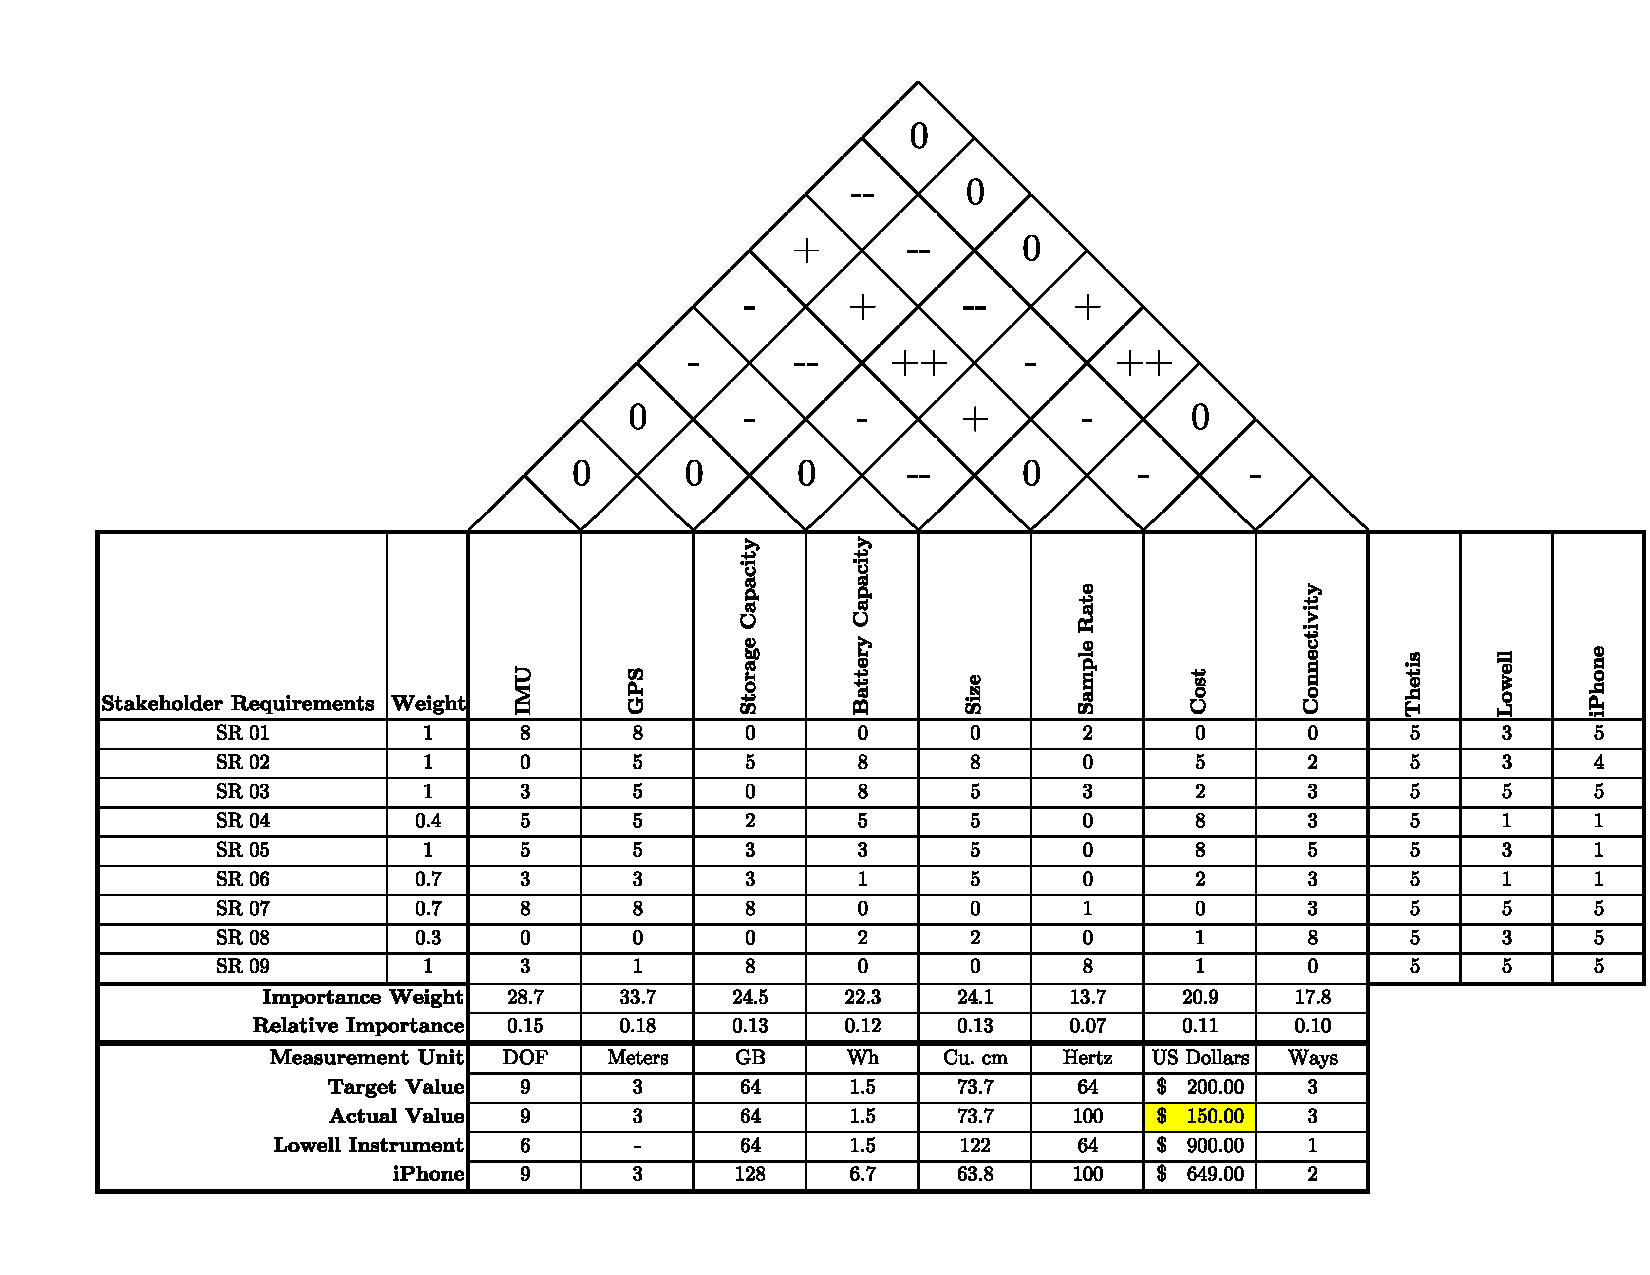
\includegraphics[height=\textwidth-24pt]{../include/ThetisHOQ.pdf}
	\end{table}
\end{landscape}

\section{Concept of Operations} \label{sec:conops}
Thetis is envisioned to be an all-in-one data logging solution that can provide real-time calculations of body orientation and position in real-time at a low cost.
In a normal operating case, Thetis will be placed near the center of gravity of a body and turned on to begin recording.
The user can then connect Thetis to a larger wireless network or use its local WiFi access point to monitor the system and adjust configuration settings.

\section{capabilities} \label{sec:capabilities}
Based on the stakeholder requirements and concept of operations, a series of capabilities were derived that influenced the subsystem and component-level requirements.
These capabilities were organized into three categories:

{
\renewcommand{\descriptionlabel}[1]{\hspace{\labelsep}\textbf{#1}}
\begin{description}
    \item[Threshol:] The bare minimum features the system needs to be have to be considered ``successful'' or ``delivered''.
    
    \item[Reach:] Features that enhance the product for the stakeholders and end users that require a moderate amount of effort above a threshold feature.						
    
    \item[Stretch:] Features that would distinguish the project from competitors and add immense value for stakeholders and end users, but come at a steep development cost in terms of time and money.
\end{description}
}

The capabilities were organized into a traceability matrix (more information in Appendix \ref{chap:traceability_matrix}), which is shown in Table \ref{tab:capabilities}.

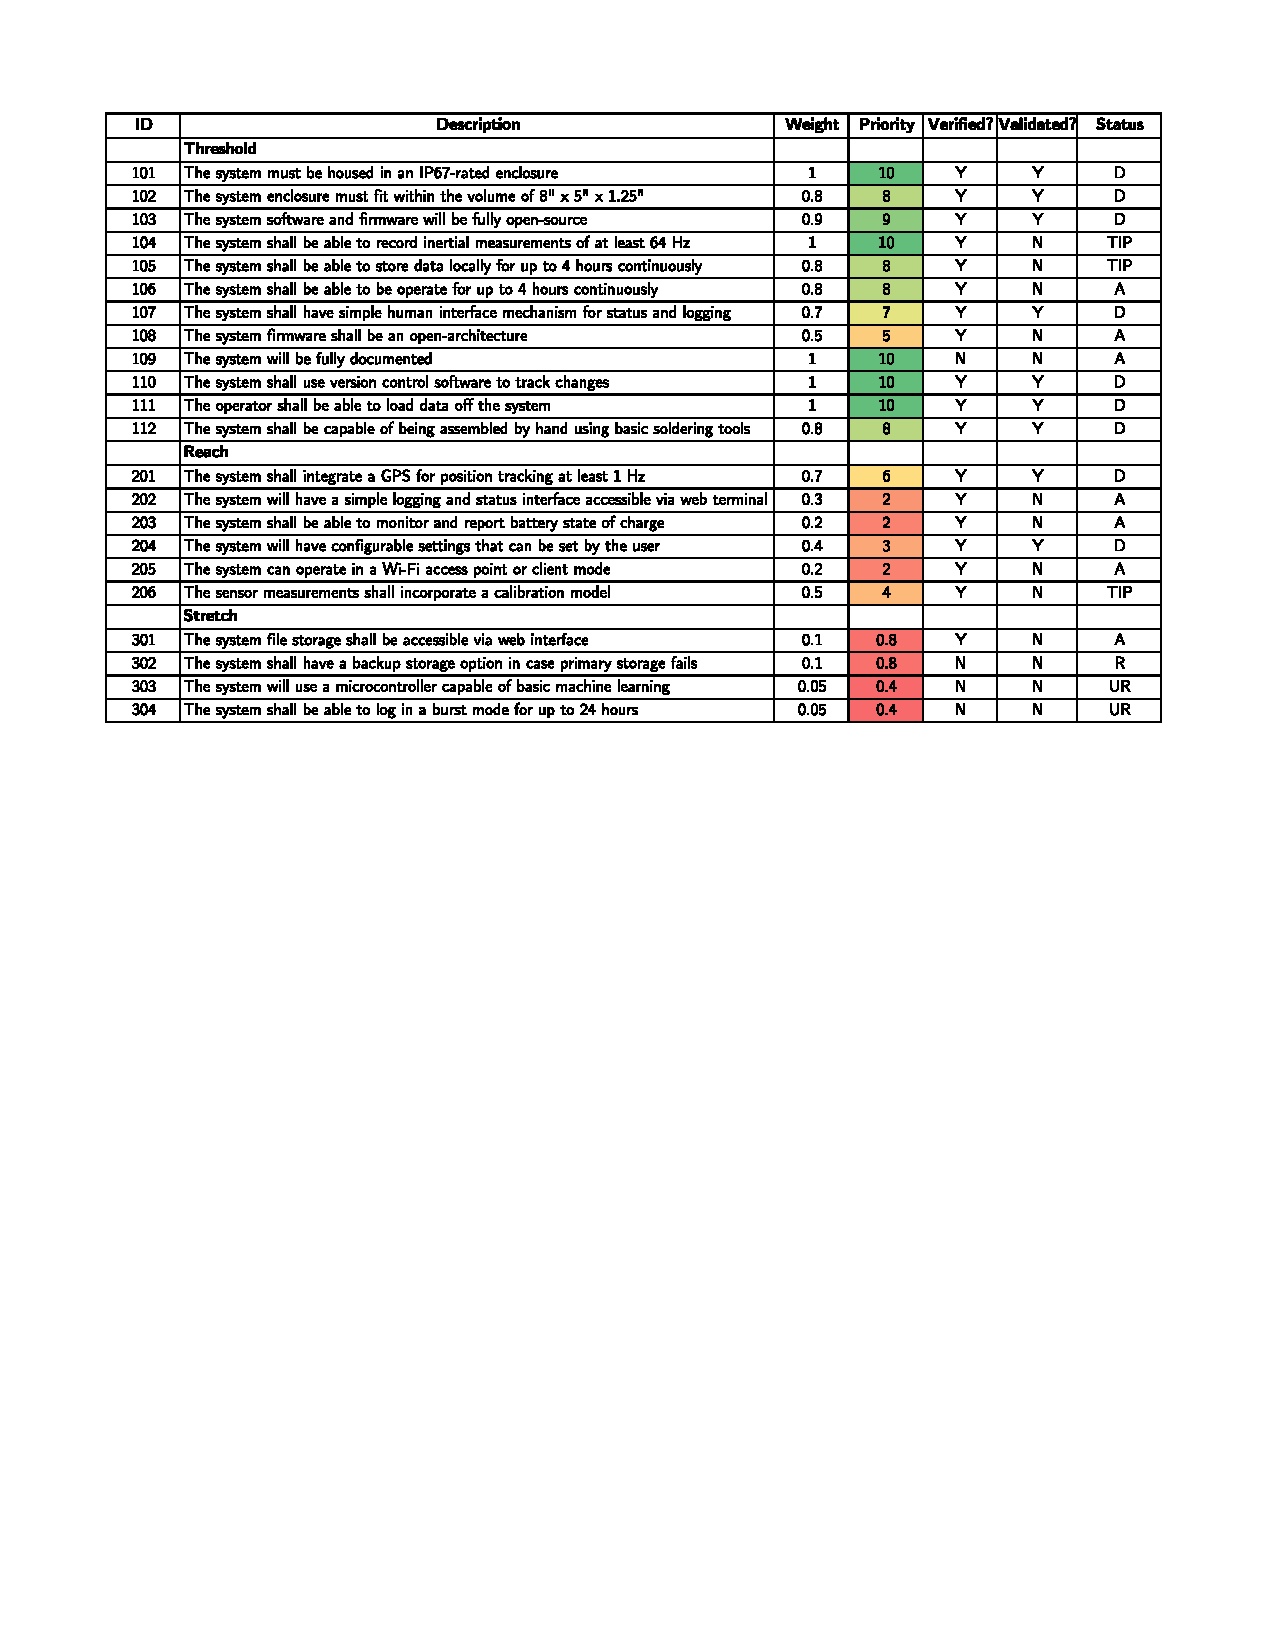
\includepdf[landscape=false, page=-, width=\textheight, offset=0 -0in, pagecommand={}]{../include/ThetisCapabilities.pdf}

% \begin{center}
% 	\renewcommand{\arraystretch}{1.5} % Set row height
% 	\begin{longtable}{| c | p{0.35\textwidth} | c | c | c | c | c |}
% 		% \caption{Thetis capabilities organized in a traceability matrix.} \\

% 		\hline
% 		\textbf{ID} & \multicolumn{1}{c|}{\textbf{Description}} & \textbf{Weight} & \textbf{Priority} & \textbf{Verified?} & \textbf{Validated?} & \textbf{Status} \\
% 		\hline
% 		& \textbf{Threshold} & & & & & \\
% 		101 & The system must be housed in an IP67-rated enclosure & 1 & 10 & Y & Y & D \\
% 		102 & The system enclosure must fit within the volume of 8" x 5" x 1.25" & 0.8 & 8 & Y & Y & D \\
% 		103 & The system software and firmware will be fully open-source & 0.9 & 9 & Y & Y & D \\
% 		104 & The system shall be able to record inertial measurements of at least 64 Hz & 1 & 10 & Y & N & TIP \\
% 		105 & The system shall be able to store data locally for up to 4 hours continuously & 0.8 & 8 & Y & N & TIP \\
% 		106 & The system shall be able to be operate for up to 4 hours continuously & 0.8 & 8 & Y & N & A \\
% 		107 & The system shall have simple human interface mechanism for status and logging & 0.7 & 7 & Y & Y & D \\
% 		108 & The system firmware shall be an open-architecture & 0.5 & 5 & Y & N & A \\
% 		109 & The system will be fully documented & 1 & 10 & N & N & A \\
% 		110 & The system shall use version control software to track changes & 1 & 10 & Y & Y & D \\
% 		111 & The operator shall be able to load data off the system & 1 & 10 & Y & Y & D \\
% 		112 & The system shall be capable of being assembled by hand using basic soldering tools & 0.8 & 8 & Y & Y & D \\
% 		\hline
% 		& \textbf{Reach} & & & & & \\
% 		201 & The system shall integrate a GPS for position tracking at least 1 Hz & 0.7 & 6 & Y & Y & D \\
% 		202 & The system will have a simple logging and status interface accessible via web terminal & 0.3 & 2 & Y & N & A \\
% 		203 & The system shall be able to monitor and report battery state of charge & 0.2 & 2 & Y & N & A \\
% 		204 & The system will have configurable settings that can be set by the user & 0.4 & 3 & Y & Y & D \\
% 		205 & The system can operate in a Wi-Fi access point or client mode	& 0.2 & 2 & Y & N & A \\
% 		206 & The sensor measurements shall incorporate a calibration model & 0.5 & 4 & Y & N & TIP \\
% 		\hline
% 		& \textbf{Stretch} & & & & & \\
% 		301 & The system file storage shall be accessible via web interface	& 0.1 & 0.8 & N & N & A \\
% 		302 & The system shall have a backup storage option in case primary storage fails & 0.1 & 0.8 & N & N & R \\
% 		303 & The system will use a microcontroller capable of basic machine learning & 0.05 & 0.4 & N & N & UR \\
% 		304 & The system shall be able to log in a burst mode for up to 24 hours & 0.05 & 0.4 & N & N & UR \\
% 		\hline

% 		\label{tab:capabilities}
% 	\end{longtable} 
% \end{center}

\section{Conceptual Design} \label{sec:conceptual_design}
The general design of the Thetis instrumentation package was built around the principles of capability, manufacturability, and affordability.
The parts selected for the design had to offer a suite of capabilities that would enable a wide range of projects.
While Thetis was designed primarily for monitoring the movement of floating bodies, it can be adapted for use in general robotics, embedded AI research, and other datalogging tasks.
Thetis is also envisioned to be continued by other endeavoring students, so it has to be easily manufacturable with a single-sided design that can be assembled by hand using tweezers and a hot-air gun.
All of this had to be designed with low-cost readily-available components in mind.
Thetis was originally designed at the start of the global chip shortage in 2020, so parts were limited in choice, especially the IMU.
It is also assumed that Thetis will be lost at some point during testing.
This is just an inevitability during field work, so keeping the cost down would also reduce the impact of such a loss on a project's budget.

\subsection{System Requirements} \label{ssec:system_requirements}
To guide Thetis' design, a series of system requirements were generated that would need to be met in order to declare the design as ``delivered''.
These requirements were derived from the House of Quality (Table \ref{tab:hoq}) and the stakeholder requirements (Section \ref{ssec:stakeholder_reqs}).
Each requirement is categorized into subsections and given a numerical designation.
The requirement is then given as a clear statement of fact with only one consideration given per requirement.
A comment may be associated with each requirement that provides additional context or relevant information.
These requirements arranged within a traceability matrix, explained in-depth in Appendix \ref{chap:traceability_matrix}						

Below is a table describing the system requirements for the Thetis instrumentation package.

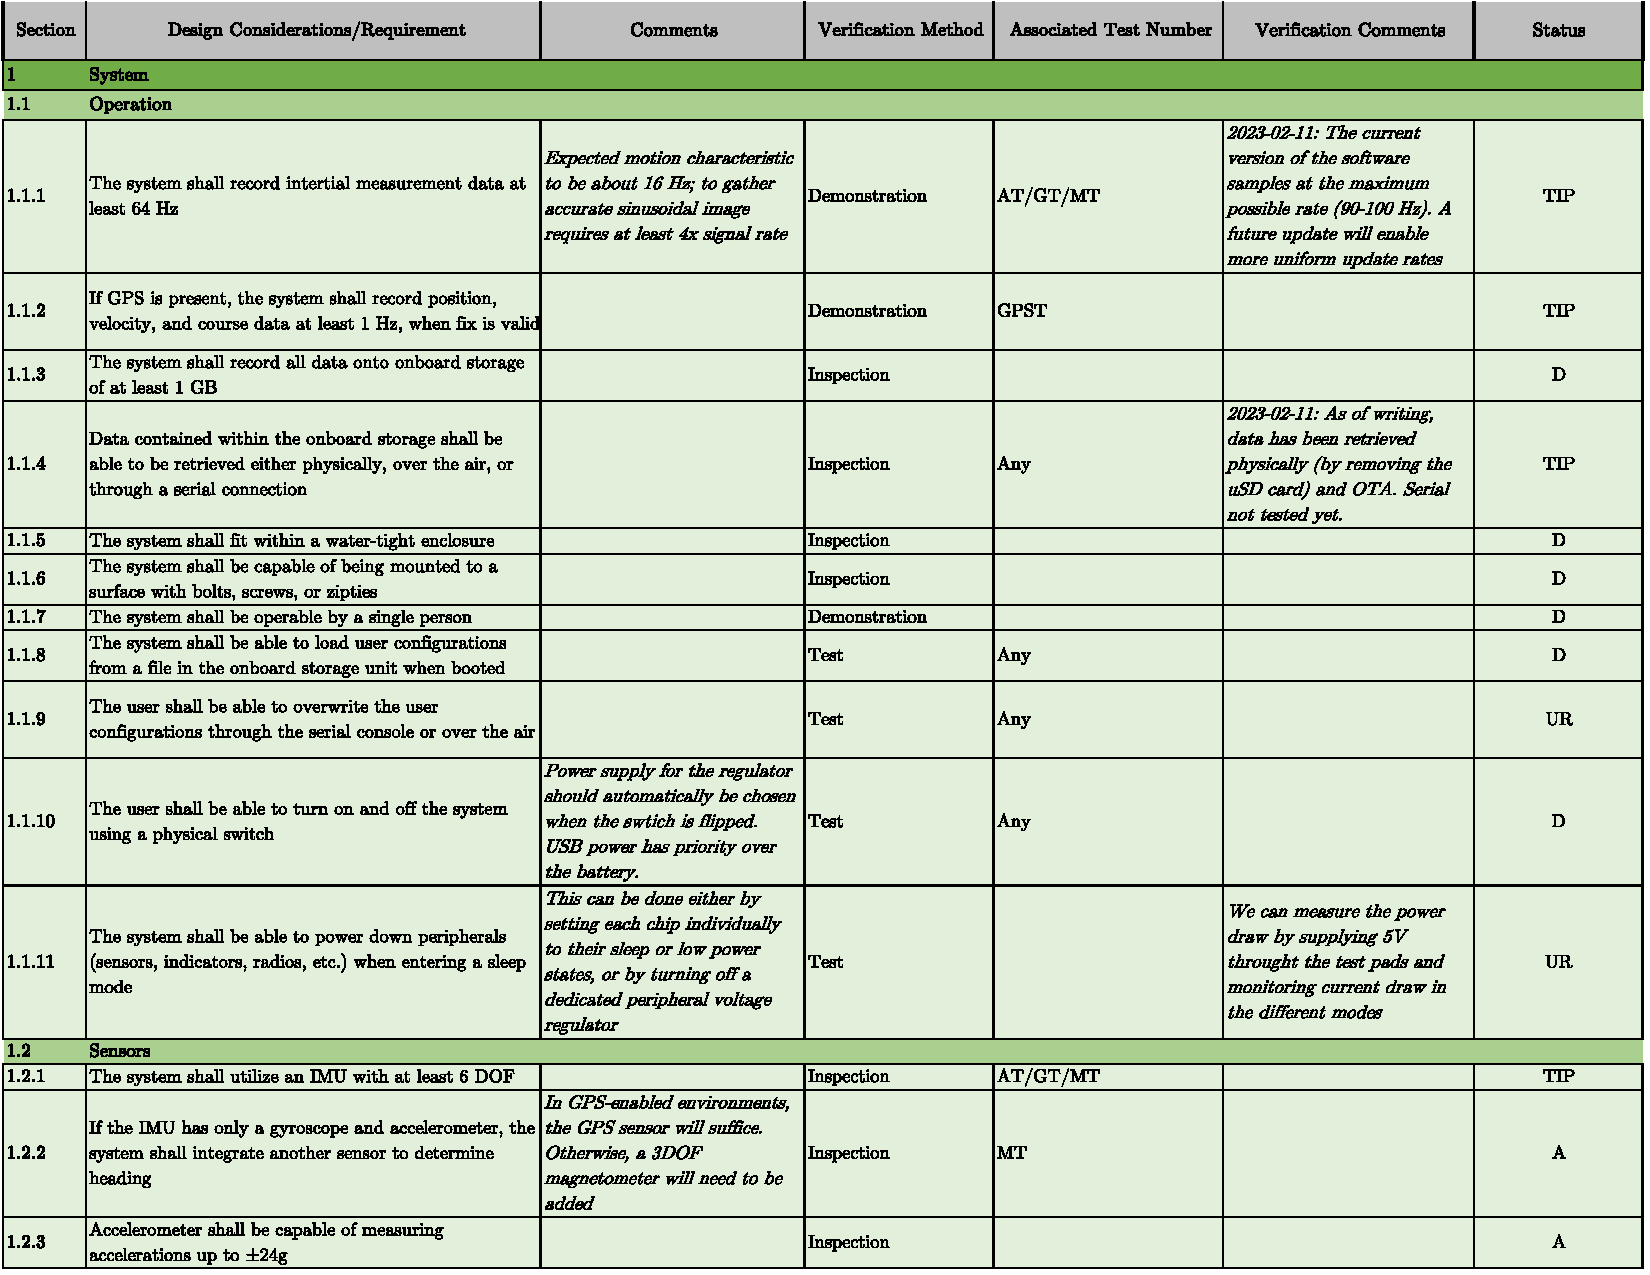
\includepdf[landscape=true, page=-, width=\textheight, offset=0 -0in, pagecommand={}]{../include/ThetisReqs.pdf}

\subsection{Failure Mode, Effect, and Criticality Analysis} \label{ssec:fmeca}
Since Thetis is intended to be used by end users who may not have a solid background in programming or electrical skills, it is important to identify potential flaws in the design and attempt to mitigate them.
Each potential flaw is given a probability of occurrence and a weighting from 0 to 10 inclusive for its severity. 
By multiplying these two values together, a Risk Priority Number (RPN) is created that highlights the severity of a potential failure mode. The RPNs are categorized into three groupings:

\paragraph*{LOW} These are RPNs with a value below 2.5 and represent little risk to the system. 
These are denoted with green highlights in the FMECA chart below.

\paragraph*{MEDIUM} These are RPN's between 2.5 and 7.5 that are represented with yellow highlights below.
Typically, these failure modes represent a noticeable threat to the system and the mitigations should be carefully implemented.

\paragraph*{HIGH} These are the highest risk RPNs between 7.5 and 10 and are represented with red highlights.
They are the most severe and should be mitigated at all cost during and after the product development cycle.

The probabilities are generally conjured from past experience, the failure ratings of parts, and other factors that are carefully mapped out and documented over time.
However, since Thetis is using hobby-grade materials and failures are not generally well-documented for the parts, the probabilities represented herein are my best guess based on experience.
The same applies for the criticality score for each potential failure.

% \begin{landscape}
% 	\begingroup
% 		\label{tab:fmeca}
% 		\centering
% 		% \vspace*{-1in}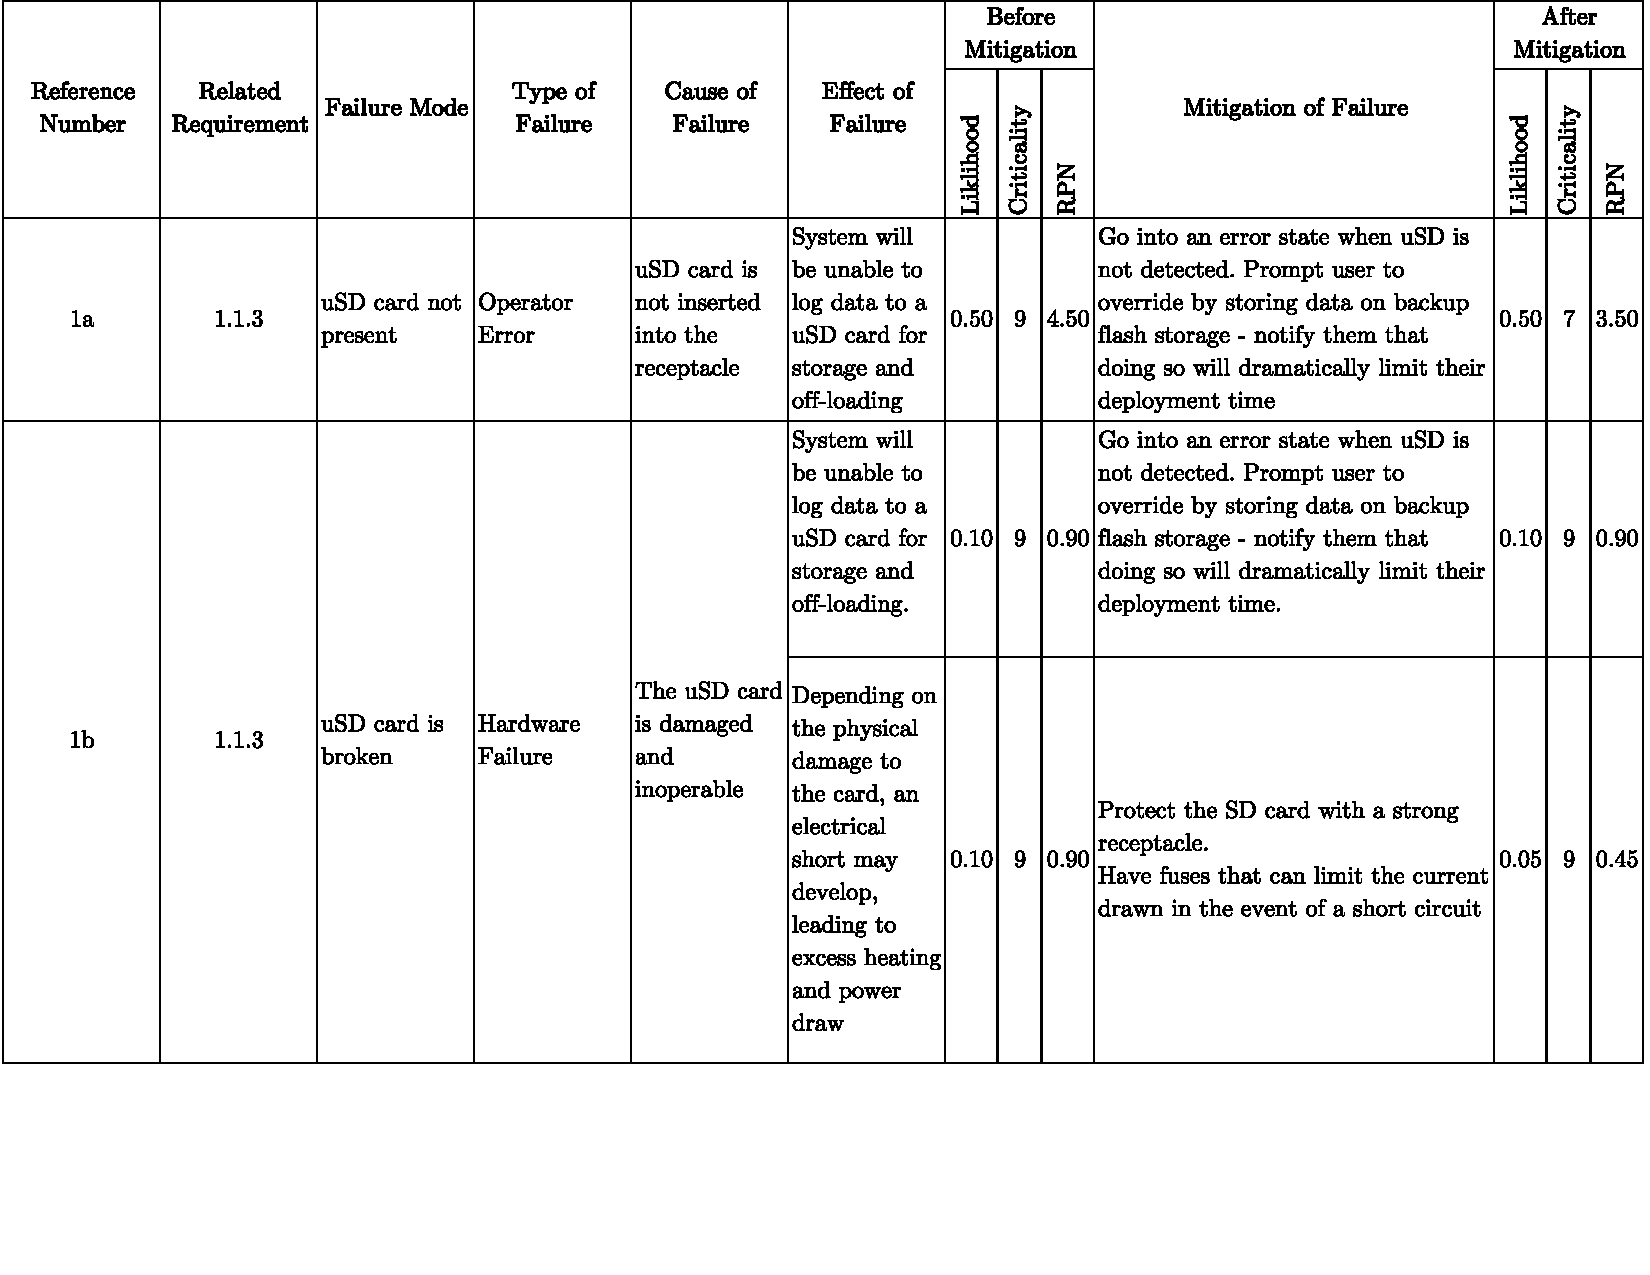
\includegraphics[trim={0 0 0 0}, height=6.75in, page=1]{../include/ThetisFMECA.pdf}
% 		% \vspace*{-1in}\captionof{table}[Failure Mode, Effect, and Criticality Analysis]{A summary of all possible failure modes and their expected effects, likelihoods, criticalities, and mitigations on the Thetis system.}
% 		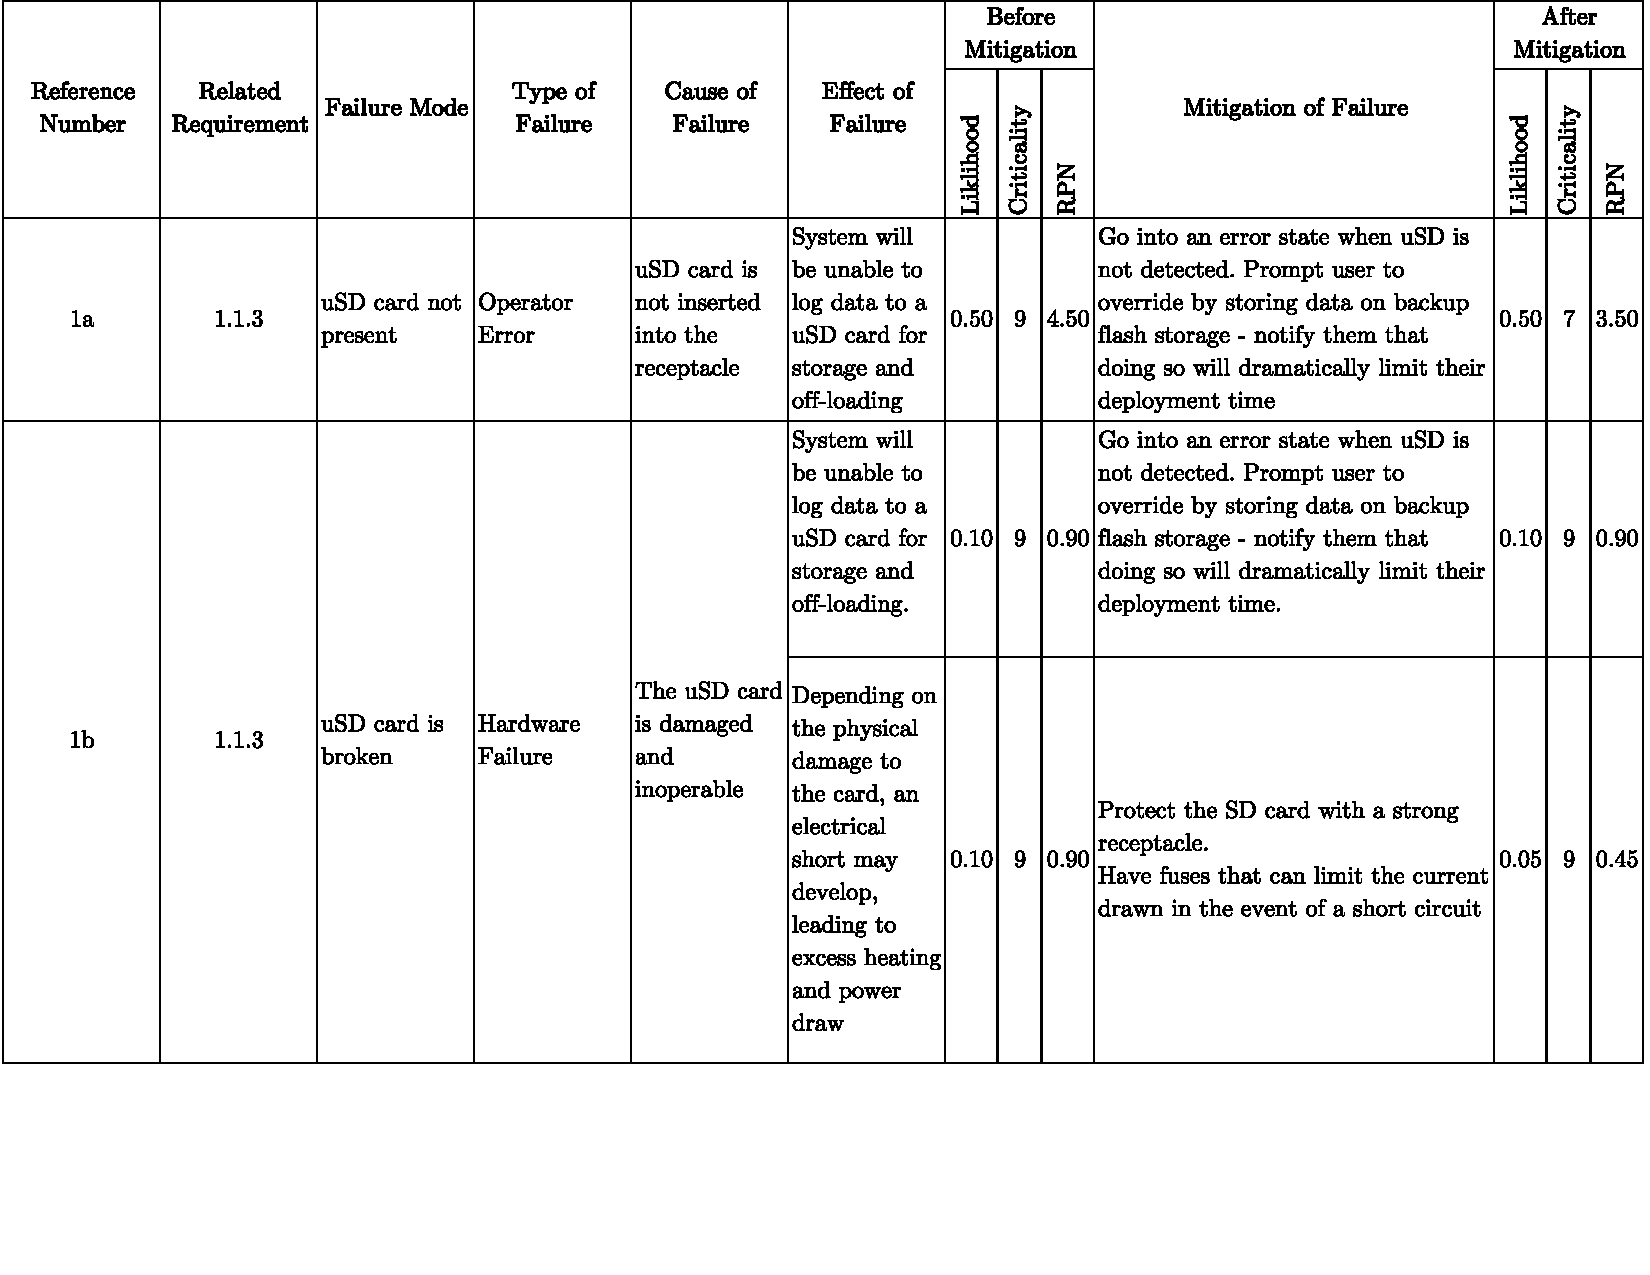
\includegraphics[height=6.75in, page=1]{../include/ThetisFMECA.pdf}
% 		\newpage
% 		\includegraphics[height=6.75in, page=2]{../include/ThetisFMECA.pdf}
% 		\newpage
% 		\includegraphics[height=6.75in, page=3]{../include/ThetisFMECA.pdf}
% 		\newpage
% 		\includegraphics[height=6.75in, page=4]{../include/ThetisFMECA.pdf}
% 		\newpage
% 		\includegraphics[height=6.75in, page=5]{../include/ThetisFMECA.pdf}
% 		% \newpage
% 		% \includegraphics[height=6.75in, page=6]{../include/ThetisFMECA.pdf}
% 	\endgroup
% \end{landscape}

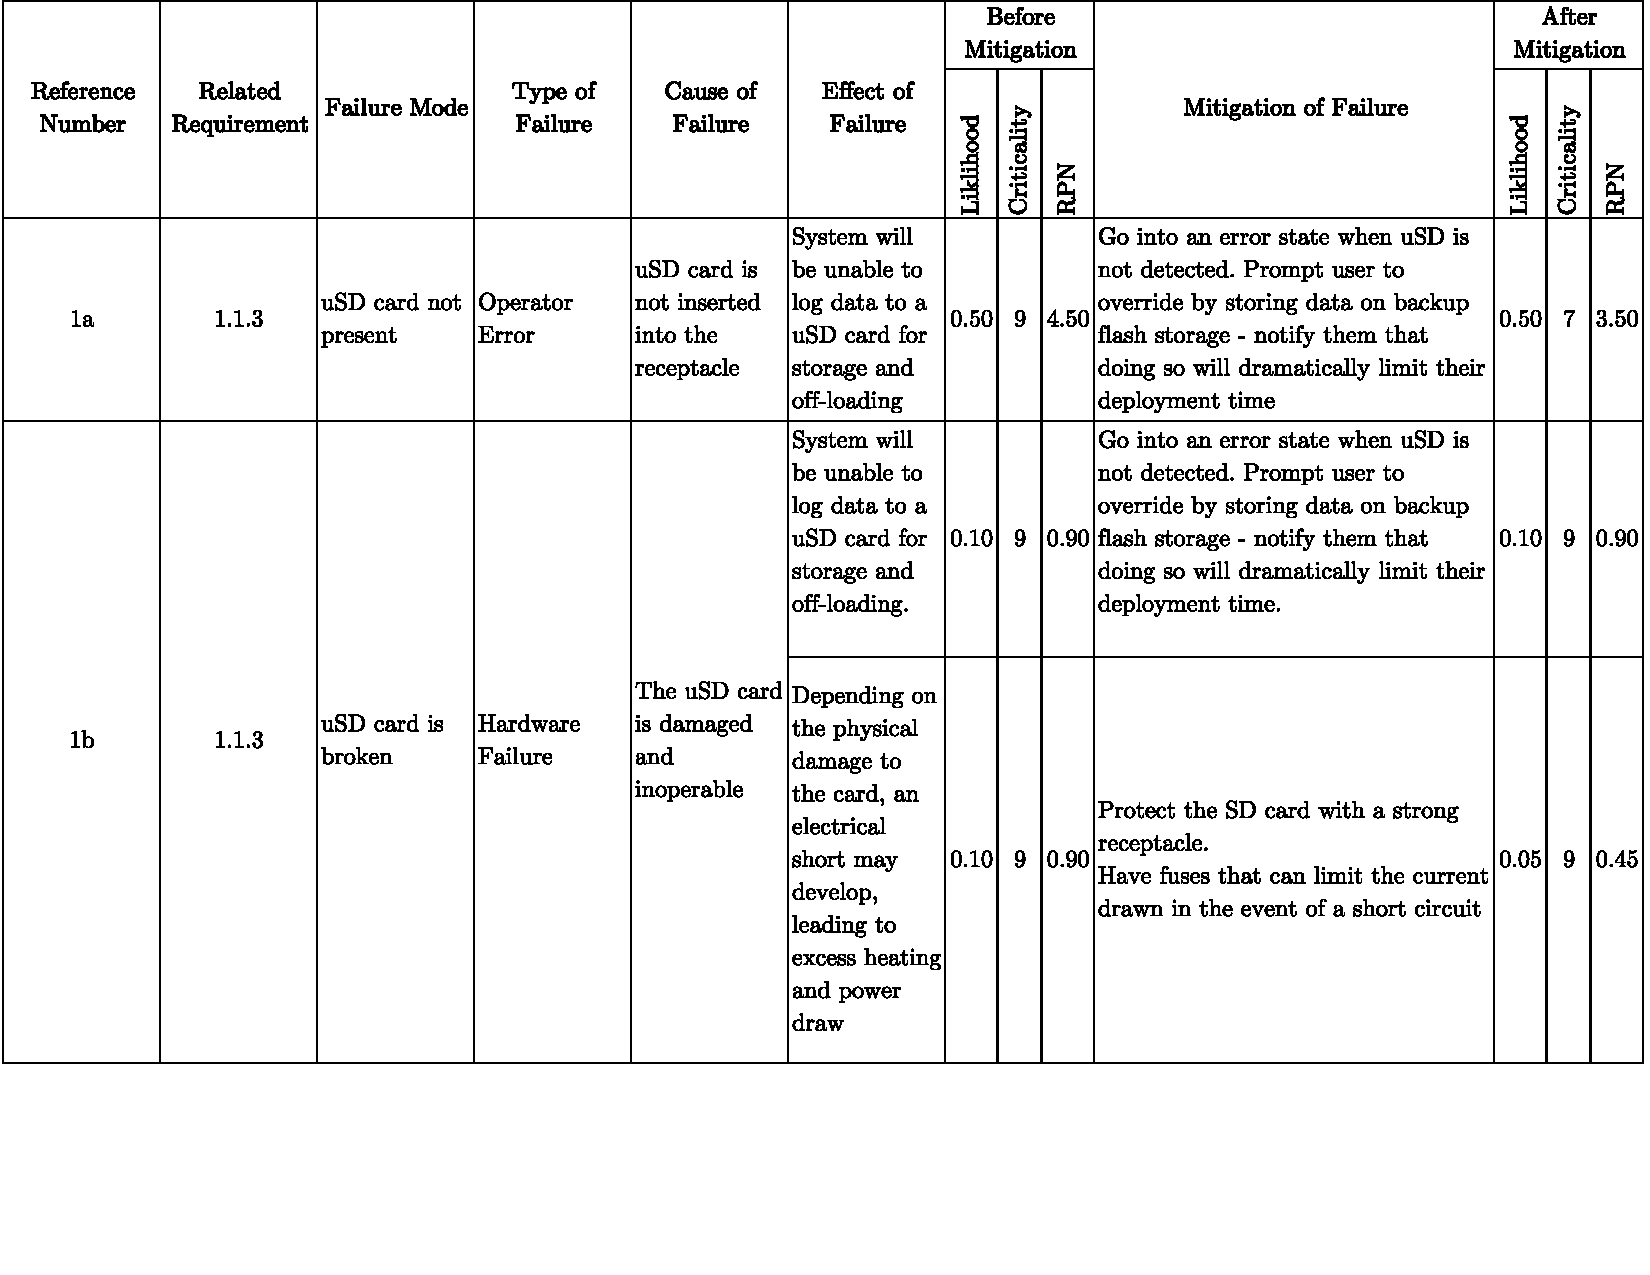
\includepdf[landscape=true, page=-, width=\textheight, offset=0 -0in, pagecommand={}]{../include/ThetisFMECA.pdf}

\subsection{Functional Block Diagram} \label{ssec:block_diagram}
Factoring in the design principles of capability, manufacturability, and affordability, along with the stakeholder requirements listed in Section \ref{ssec:stakeholder_reqs}, a block diagram was constructed that integrated the crucial parts and drew out their interactions.
This block diagram shows the data sharing relationships in blue and the power relationships in warm colors.
Labels on the specific lines indicate the specific communication protocol or voltage level being used by the line.
Explanations for these protocols and acronyms can be found in the Appendix.

\begin{figure}[h!]
	\label{fig:thetis_block_diagram}
	\caption[Thetis RevF5 Block Diagram]{A block diagram representation of the Thetis RevF5 instrumentation board.}
	\centering
	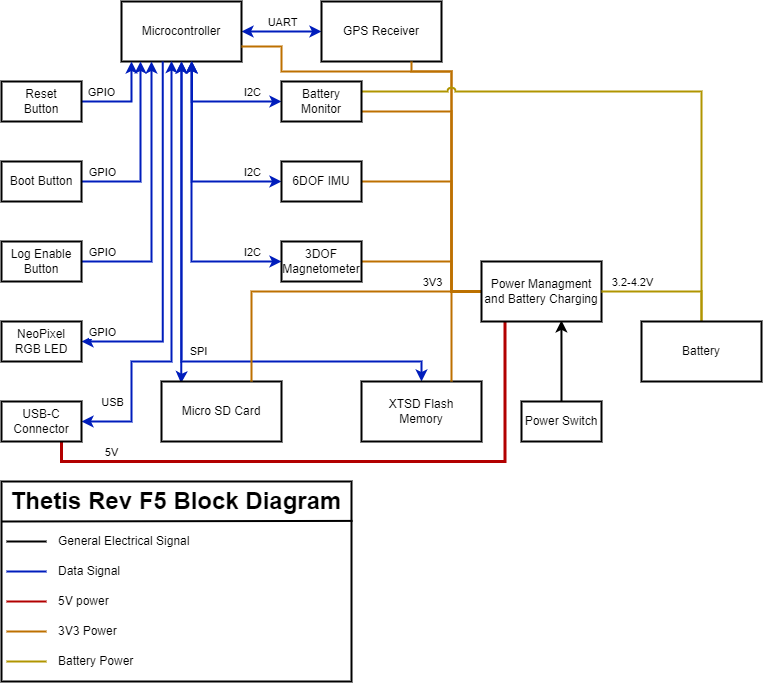
\includegraphics[width=5in]{design/block_diagram.png}
\end{figure}

\subsection{Functional Flow Diagram} \label{ssec:flow_diagram}
Based off the block diagram and interviews with potential end users, a notional flow diagram for the firmware was created.
The code was designed to be modular and allow for new features to be quickly added or removed with separate libraries.

\begin{figure}[h!]
	\label{fig:thetis_flow_diagram}
	\caption[Base Firmware Flow Diagram]{A flow diagram representation of the base firmware of the Thetis instrumentation board.}
	\centering
	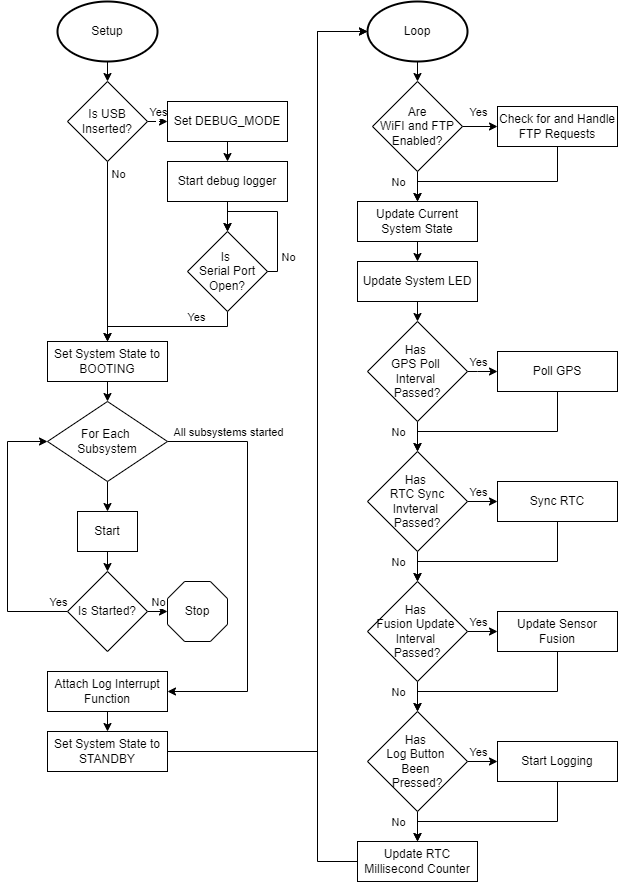
\includegraphics[width=5in]{design/flow_diagram.png}
\end{figure}

\section{Brief Revision History} \label{sec:revision_history}
After carefully considering all the design criteria from the stakeholder requirements and system requirements, Thetis began several design revisions.
The first design revision, Rev F1, was a functional proof of concept.
It incorporated many of the base design features of later Thetis revisions, but relied on a breakout board for the IMU mounted to the bottom of the board and had the battery placed on top.
This forced the battery to be smaller than the desired capacity and overfilled the enclosure, causing excessive compression and stress when the enclosure was tightened and secured.

[INSERT IMAGE OF REVISION F1]

The next revision, F2, changed to a new microcontroller version that simplified the circuit while providing the same capability of the previous revision.
This version also switched from a Micro SD card receptacle to a soldered SMD flash memory chip.
This chip maintained the same capacity requirements from the stakeholders, but took up a fraction of the space on the board.
However, since this chip was directly soldered to the board, the only way to offload date was through the microcontroller either through an FTP server, or through the USB interface.
This is not ideal - especially in the early testing phases, as those features are more complex to implement programmatically and test data cannot be easily offloaded if there is an issue with the microcontroller.
There were also reliability issues which manifest in force on later revisions.
This revision also kept the breakout board for the IMU on the back, giving it the same space constraint problem as its predecessor.

[INSERT IMAGE OF REVISION F2]

For Revision F3, some minor changes were made to the diagnostic LEDs and user inputs.
Several discrete LEDs for logging, error notification, and low battery, were replaced by a single addressable RGB LED that could flash different colors and patterns to convey the system state or errors.
The dedicated log enable button was also removed in favor of using the boot select button for both purposes.
However, this method was entirely flawed as the log enable button relies on an interrupt input to trigger the system to begin recording.
On the ESP32-S2 microcontroller, an interrupt tied to GPIO 0 (the boot select pin) would cause the system to crash and force a reset.
Therefore, the entire design had to be scrapped due to this design flaw.

[INSERT IMAGE OF REVISION F3]

Revision F4 was the most radical design change of the series.
It marked a migration to all SMD components (no breakout board for the IMU) and incorporated all of the design lessons from the previous revision.
However, the IMU that was used in previous revisions, the Bosch BNO055\footnote[2]{\url{https://www.digikey.com/en/products/detail/bosch-sensortec/BNO055/6136301}} was amongst the many IMUs affected by the Great Chip Shortage and was therefore unavailable.
So, this design had to adapt by incorporating a new, previously untested IMU, the STdevices LSM6DSO32\footnote[3]{\url{https://www.digikey.com/en/products/detail/stmicroelectronics/LSM6DSO32TR/11694177}}.
This new IMU does not have a magnetometer and at the time of its design, they were hard to find in stock at any distributors.
So, in anticipation of the Chip Shortage ending, the BNO055 was incorporated to the design, but not populated, giving this board the unique opportunity of having either or both IMUs present - a useful feature for more accurate sensor fusion, but a terrible prospect for software integration.
Additionally, this design reintroduced the micro SD card receptacle, but this time, the SMD flash chip was laid out beneath it.
This provided the assembler to determine which storage system they wanted: easier to use micro SD, or more resilient SMD flash.
Programmatically, these devices work the same, so the software cost was minimal while providing some flexibility.
However, this design was also fundamentally flawed as the newly reintroduced log enable button was not integrated into the design properly and the chip select pin for the storage device was connected to an incorrect controller pin.
This latter issue forced the microcontroller to crash and reset every time is tried to write to the external flash memory, necessitating a new board revision.

[INSERT IMAGE OF REVISION F4 (BOTH RENDERED AND ACTUAL)]

\section{Final Design} \label{sec:final_design}
Revision F5 is the latest version that realizes all the hardware features Thetis is meant to incorporate while being easy to assemble and use.
The BNO055 was fully removed from the system in favor of adding a dedicated magnetometer, the STdevices LIS3MDL\footnote[4]{\url{https://www.digikey.com/en/products/detail/stmicroelectronics/LIS3MDLTR/4309733}}.
By reorganizing some components, the SMD flash ship and micro SD card receptacle were placed side-by-side enabling both primary and secondary storage services, enabling backups and improving reliability.
Then, to improve the battery monitoring capabilities, a battery gauge IC was added.
The MAX17048\footnote[5]{\url{https://www.digikey.com/en/products/detail/analog-devices-inc-maxim-integrated/MAX17048G-T10/3758921}} is a monitoring IC that runs a mathematical model of the battery's discharge curve given its amp-hour capacity and current operating voltage.
This data is reported to the microcontroller as the current battery percentage or life remaining - making this a crucial part of monitoring performance and operations of Thetis when deployed.
Component types and placements were also streamlined to improve manufacturability and allow the potential for the device to be more easily assembled by a pick and place machine.
This also allows students who have never assembled PCBs before to more easily take up the task and build these boards themselves.

[INSERT IMAGE OF REVISION F5 (BOTH RENDERED AND ACTUAL)]

The next sections detail the assembly process in more detail and provide the schematics and PCB layout for Revision F5.
The schematics for the previous revisions can be found in the appendix.

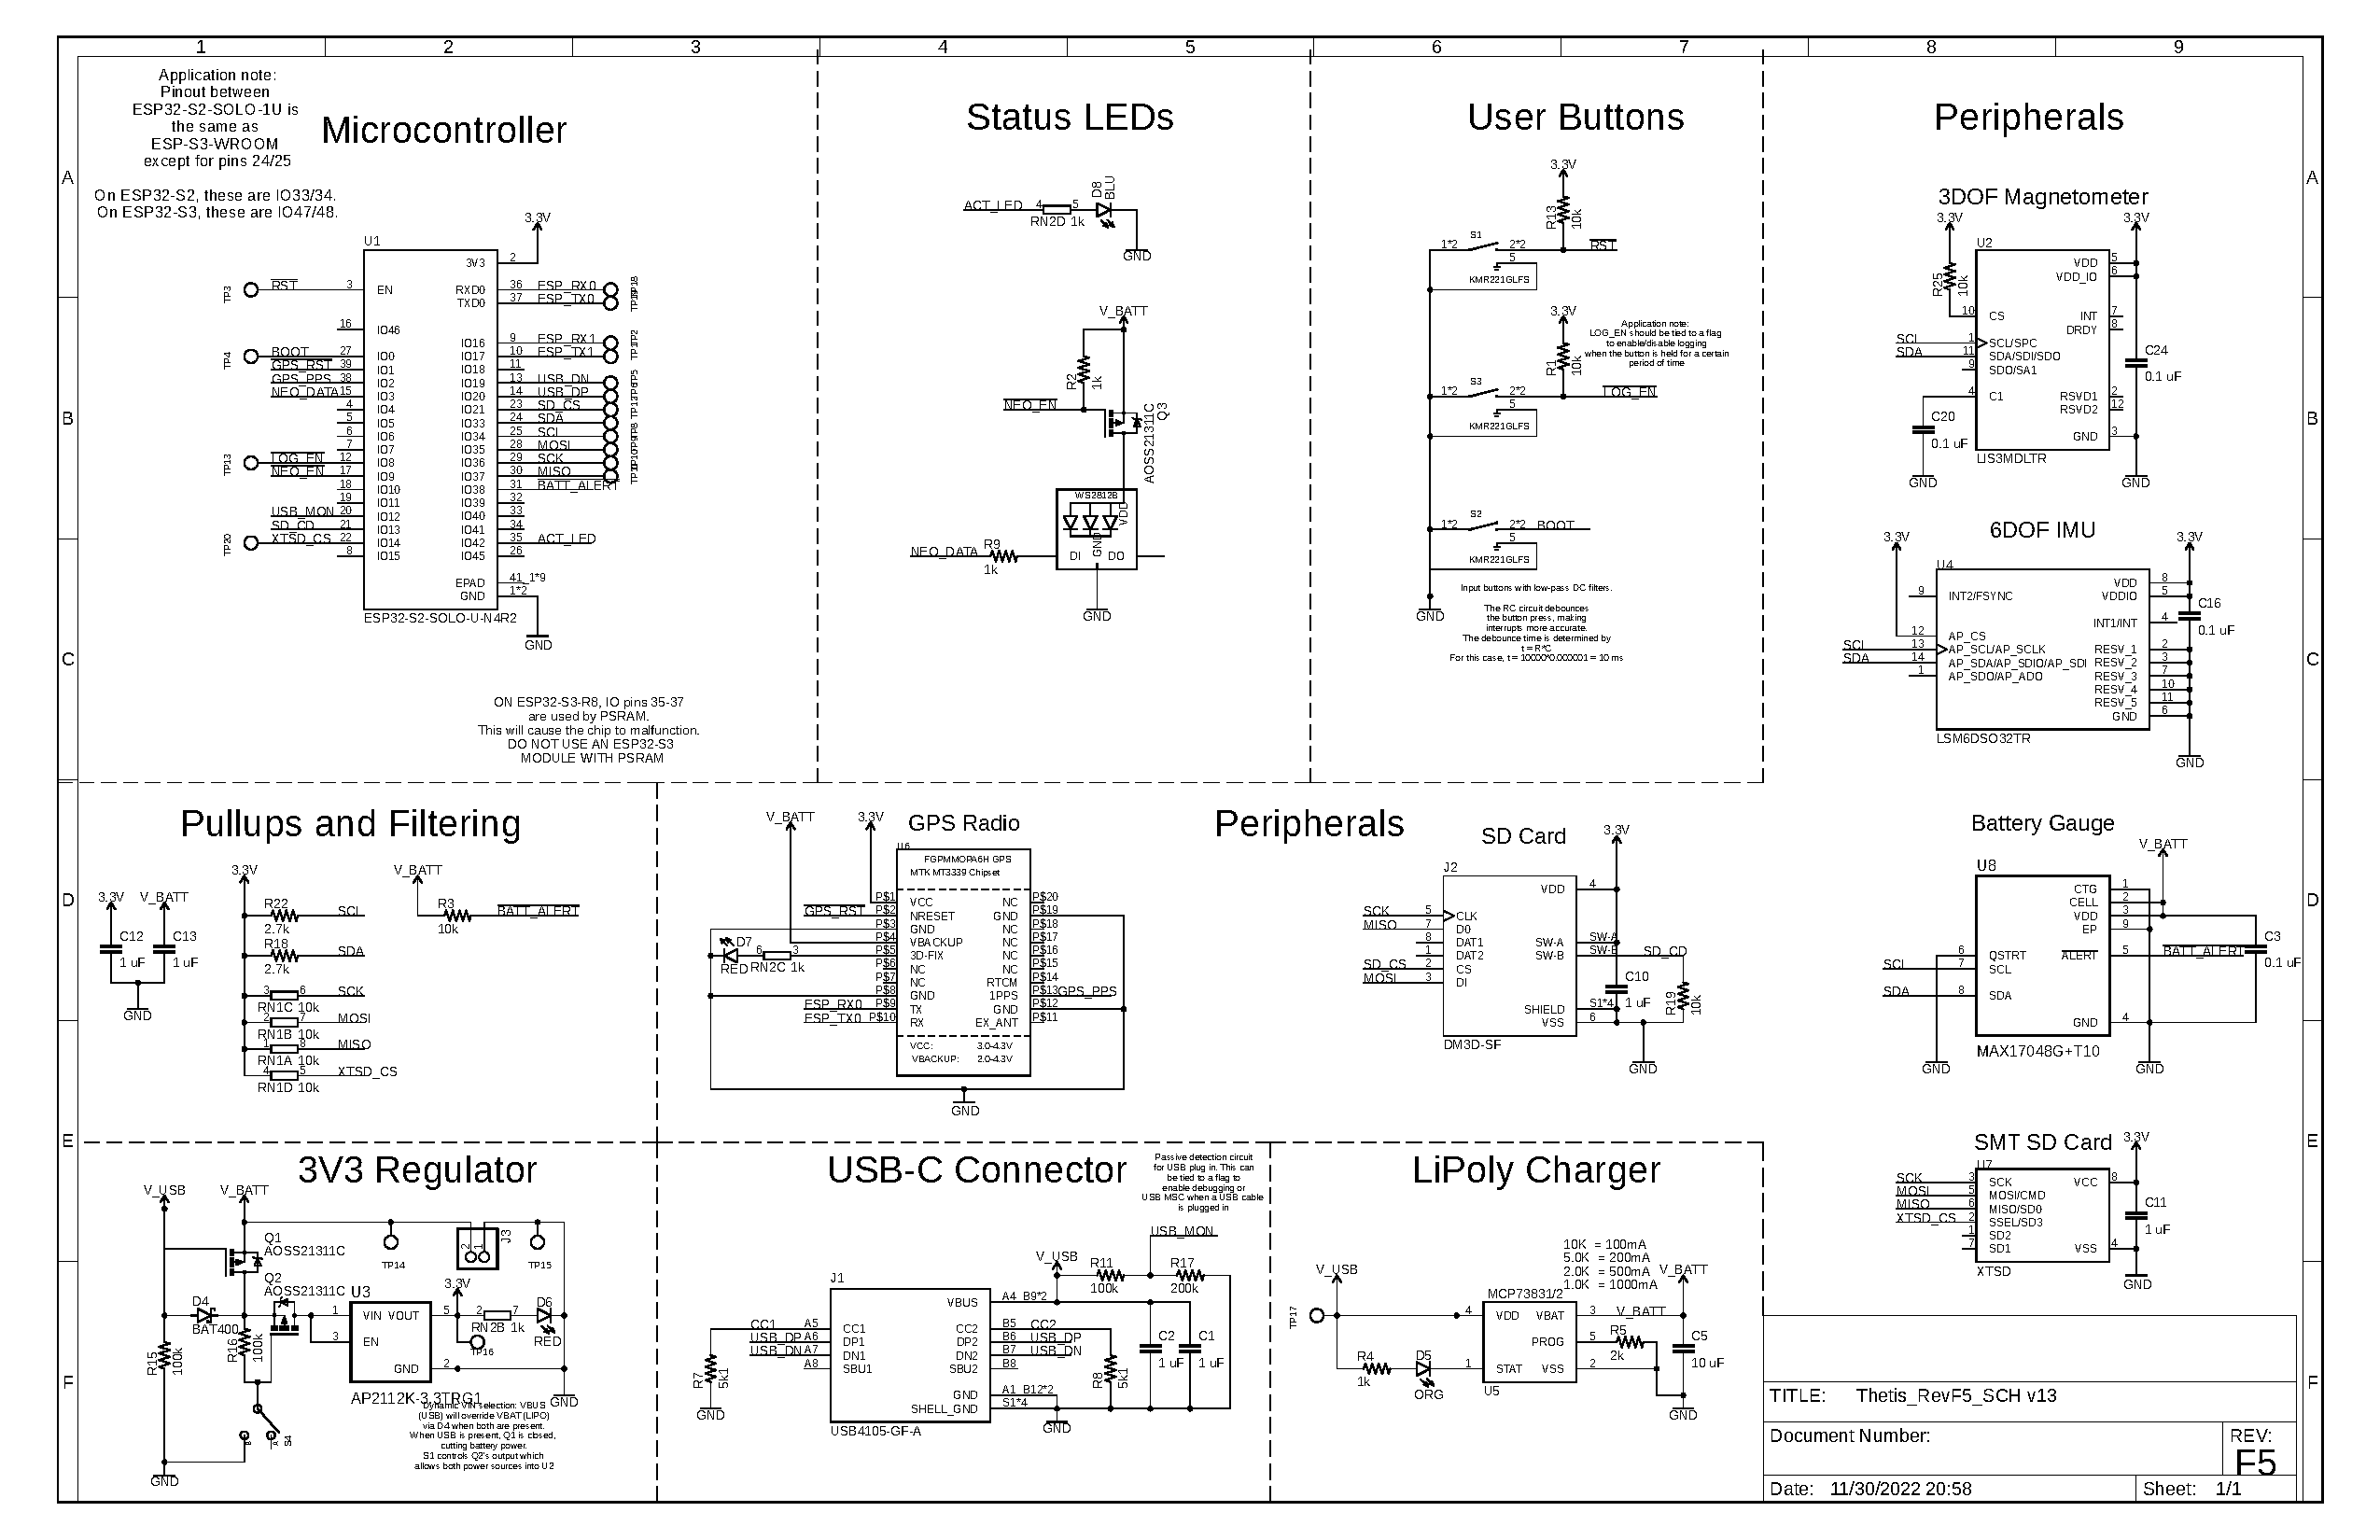
\includepdf[landscape=true, width=\textheight, offset=-0in -0.25in, pagecommand={\subsection{Schematic} \label{ssec:revf5_schematic}}]{../include/Thetis_RevF5_SCH.pdf}

\subsection{Assembly Technique} \label{ssec:assembly_techniques}
Thetis was designed with surface mount soldering as the primary assembly technique.
This technique differs from traditional soldering as the components are so small that a soldering iron is ineffective in mounting components to the board.
Many of the ICs used on the final Thetis revision do not have exposed legs or pads that can be touched with an iron, so solder paste and hot air are required.

[INSERT COMPARISON SHOT OF THROUGH HOLE AND SURFACE MOUNT SOLDERING]

\paragraph*{Solder Deposition} First, the bare PCB is placed beneath a stencil and secured with tape.
It is important that all of the pads on the PCB are aligned with the cutouts in the stencil as the solder paste must be evenly and thoroughly distributed on the board.
When the PCB is in place, a line of paste is placed on one side and smoothly dragged along the cutouts with even pressure applied throughout.
When the stencil is removed, there should be a healthy deposit of solder paste on each pad as shown in the rightmost picture of Figure \ref{fig:stencil_process}

[INSERT PICTURE SERIES SHOWING STENCIL LAYING, SOLDER PASTE APPLICATION, AND RESULTANT DEPOSIT]

\paragraph*{Component Placement} From here, components can be placed onto the PCB carefully using tweezers.
Some components measure in at tenths of an inch across and require placement tolerances of hundredths of an inch.
Thankfully, in some areas, the surface tension of the solder when melting will forgive slightly misplaced components and drag them into the appropriate spots.
However, it is important not to smear the solder as it may inadvertently bridge pads together and create shorts and undesired behavior.
Throughout assembling these boards, this particular issue was the most common during the assembly process and occurred regularly on the USB-C receptacle, and IMU ICs where the pins are close together.

\paragraph*{Reflow Soldering} When all of the components are placed, the PCB can be placed into a reflow oven for baking.
The oven used for this process uses infrared radiation to evenly heat the board through a set profile.
The temperature profile is specified by the solder paste manufacturer and gives ample time for the components to heat up and the paste to transform from a viscous mixture, to a solid metallic connection.
The entire process from putting the board beneath the stencil to assembled and ready for inspection can take anywhere from 3 hours for a novice assembler, to 45 minutes for a more experienced one.

[INSERT PICTURE SERIES SHOWING COMPONENT PLACEMENT, SOLDERING OVEN, AND FINAL RESULT]

\paragraph*{Inspection} Following a successful reflow, the board must be inspected for defects.
The most common are solder bridges between pads that create undesired shorts and can damage parts.
The inspection will also check that parts are in the correct locations and orientations and that no shorts exist between power rails and ground.
A microscope and good multimeter are crucial to this process.

If a soldering defect is discovered, the board can be placed onto a small heating plate to melt the solder and remove the part.
Then, the part can be removed and the pads on both the component and board are cleaned up using a soldering iron to ensure the proper amount of solder is present.
Once the pads are cleaned, either hot air or the heating pad can be used to heat the afflicted area and remelt the solder so the part can be replaced on the board.
The board is inspected again and if the issue is cleared, the board is ready for testing.

[INSERT A PICTURE SERIES ON INSPECTING THE ASSEMBLED BOARD, REPLACING A COMPONENT, AND THEN REINSPECTING IT]

\paragraph*{Testing} When the board passes a visual inspection and there are no power shorts present, the board is plugged into a programming computer via the USB port.
The microcontroller is placed into the bootloader mode by holding the boot button and pressing the reset button.
This should cause the microcontroller to show up as a USB device on the computer.
From here, the latest Thetis firmware can be flashed to the new board.
By default, when plugged into USB, the board enters a diagnostic testing mode that prints out the boot and initialization status.
By opening a serial console, the assembler can see this process in real time.
If there are any errors while initializing, the firmware will report which device is having a problem.
The assembler will then need to do a deeper inspection to find the cause of the error and rectify it.

[INSERT PICTURE SERIES OF BOOTING AND TESTING THE NEW BOARD]

Once the new board boots without issue, the board is ready for deployment and can be used by operators and intended end users.

% \subsection{PCB Design} \label{ssec:revf5_pcb}

% \subsection{Unit Testing} \label{ssec:unit_testing}